\chapter{Verification}
\label{verification}

With the computational approach implemented in \acrshort{moose}, an effort must be made to verify the solvers. This step is crucial to ensure the implementation is correct and to test the numerical accuracy of the methods used for both the radiation transport and mobile depletion packages. To this end, both solvers are independently verified using simple analytical solutions, benchmark problems, and the method of manufactured solutions. This chapter begins by describing the verification strategy and results for the \acrshort{sn} radiation transport solver. Following the verification of the \acrshort{sn} solver, the methods used to mitigate ray effects are verified. Finally, the verification scheme employed for the mobile depletion solver is discussed.

\section{Discrete Ordinates Radiation Transport}
\label{verification:radiation_transport_sn}

The verification of the \acrshort{sn} radiation transport implementation was performed using a simple transport problem to test the space-angle convergence of these methods. This was followed by the use of a series of standard transport benchmark problems, the Kobayashi problems \cite{kobayashi_benchmarks}. While these verification cases are useful to prove the correctness of mono-energetic radiation transport problems, they do not consider the energy dependence of the transport equation. To assess the performance of the transport solver in the multi-group case, a new benchmark problem is proposed using the planned Ontario Tech subcritical assembly.

\subsection{1D Analytical Transport Problem}
\label{verification:radiation_transport_sn:1D_anal}

Consider a 1D infinite slab absorber with a planar particle source placed at $x = 5$ cm emitting isotropically in all directions. The radiation transport equation for this case can be written as the following:
\begin{equation}\label{eq:slab_transport}
    \mu\frac{d}{dx}\psi(x, \mu) + \Sigma_{t}\psi(x,\mu) = \frac{q}{2}\delta(x - 5),\,\,\,\,x\in[-\infty, \infty],\mu\in[-1, 1]\text{.}
\end{equation}
The solution to Eq.~\ref{eq:slab_transport} takes the following form \cite{computational_methods}:
\begin{equation}\label{eq:slab_transport_solution}
    \Phi_{a}(x) = \int_{-1}^{1} \psi(x,\mu)\,d\mu = \frac{q}{2}E_{1}(\Sigma_{t}|x - 5|)\text{,}
\end{equation}
where $E_{1}$ is the exponential integral function of the first kind:
\begin{equation}\label{eq:exp_integral}
    E_{1}(\Sigma_{t}|x - 5|) = \int_{1}^{\infty}\frac{e^{-\Sigma_{t}|x - 5| \gamma}}{\gamma}\,d\gamma\text{;}
\end{equation}
this problem is modelled in \acrshort{gnat} as the first verification problem. This particular problem was chosen for the injection of a strong heterogeneity through the slab radiation source. This work sets the source to $q = 1.0$ s\textsuperscript{-1} and $\Sigma_{t}$ is set to $0.1$ cm\textsuperscript{-1}. An important consideration for this benchmark problem is that the analytical solution is singular as one approaches the slab source:
\begin{equation}
    \lim_{x\rightarrow 5}\frac{q}{2}E_{1}(\Sigma_{t}|x - 5|) = \infty\text{.}
\end{equation}

The numerical solution to this problem applies vacuum boundary conditions at $x = 0$ cm and $x = 10$ cm to emulate the effect of the infinite slab. The domain is meshed with either 10, 100, or 1000 elements with linear Lagrange basis functions. A Legendre quadrature rule is used with either 10, 20, or 40 directions per octant of the unit sphere, resulting in 20, 40, or 80 total directions in 1D as there are two octants of the unit sphere in infinite slab geometry. The \acrfull{pjfnk} solver was used with block Jacobi preconditioning. The largest initial residual vector magnitude across all refinement cases reported by \acrshort{petsc} is $9.974811$, and so a relative convergence convergence criteria of $10^{-8}$ was used. This was found to be sufficient for localizing sources of error to the spatial and angular discretization scheme as further decreases in the relative convergence criteria did not result in substantial changes to the numerical solution. The numerical fluxes, analytical fluxes, and the absolute relative error between the numerical and analytical fluxes can be found in Figures~\ref{fig:verification:1D_flux_10_elem} to \ref{fig:verification:1D_flux_1000_elem}. Both are plotted over the range from $x = 5$ cm to $x = 10$ cm.

\begin{figure}[H]
    \centering
    %\hfill
    \begin{subfigure}[b]{0.495\textwidth}
        \centering
        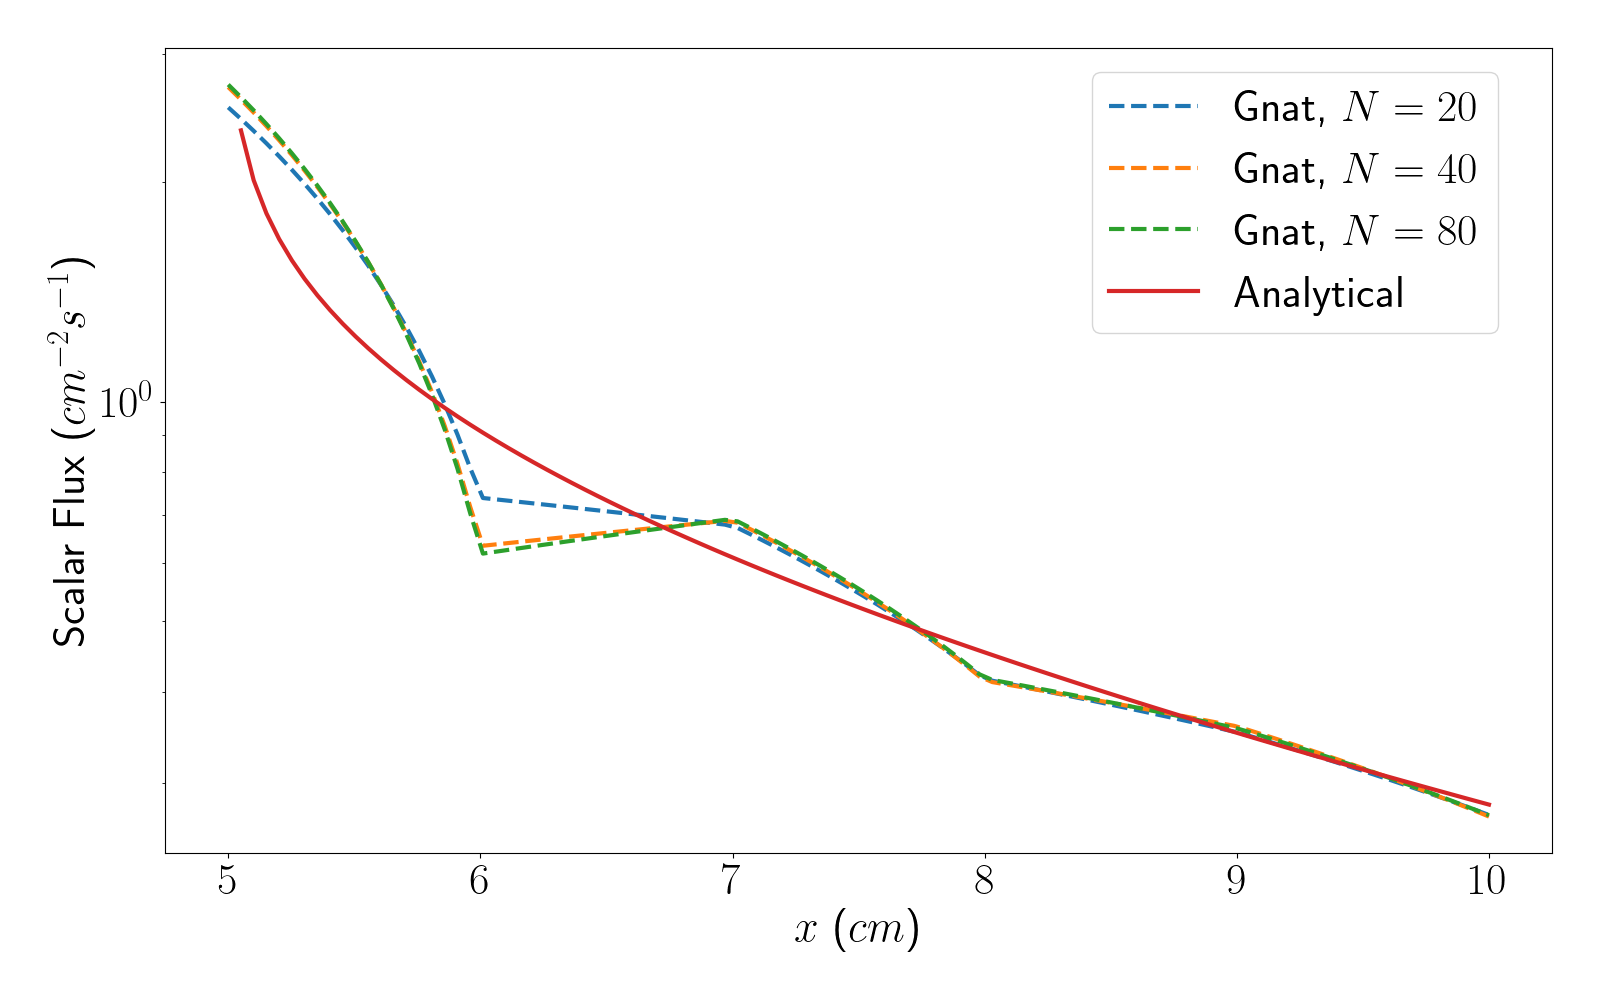
\includegraphics[width=\textwidth]{images/verification/1d_slab/1D_analytical_flux_1.png}
        \caption{Numerical and analytical scalar fluxes.}
        \label{fig:verification:1D_flux:10_elem}
    \end{subfigure}
    \hfill
    \begin{subfigure}[b]{0.495\textwidth}
        \centering
        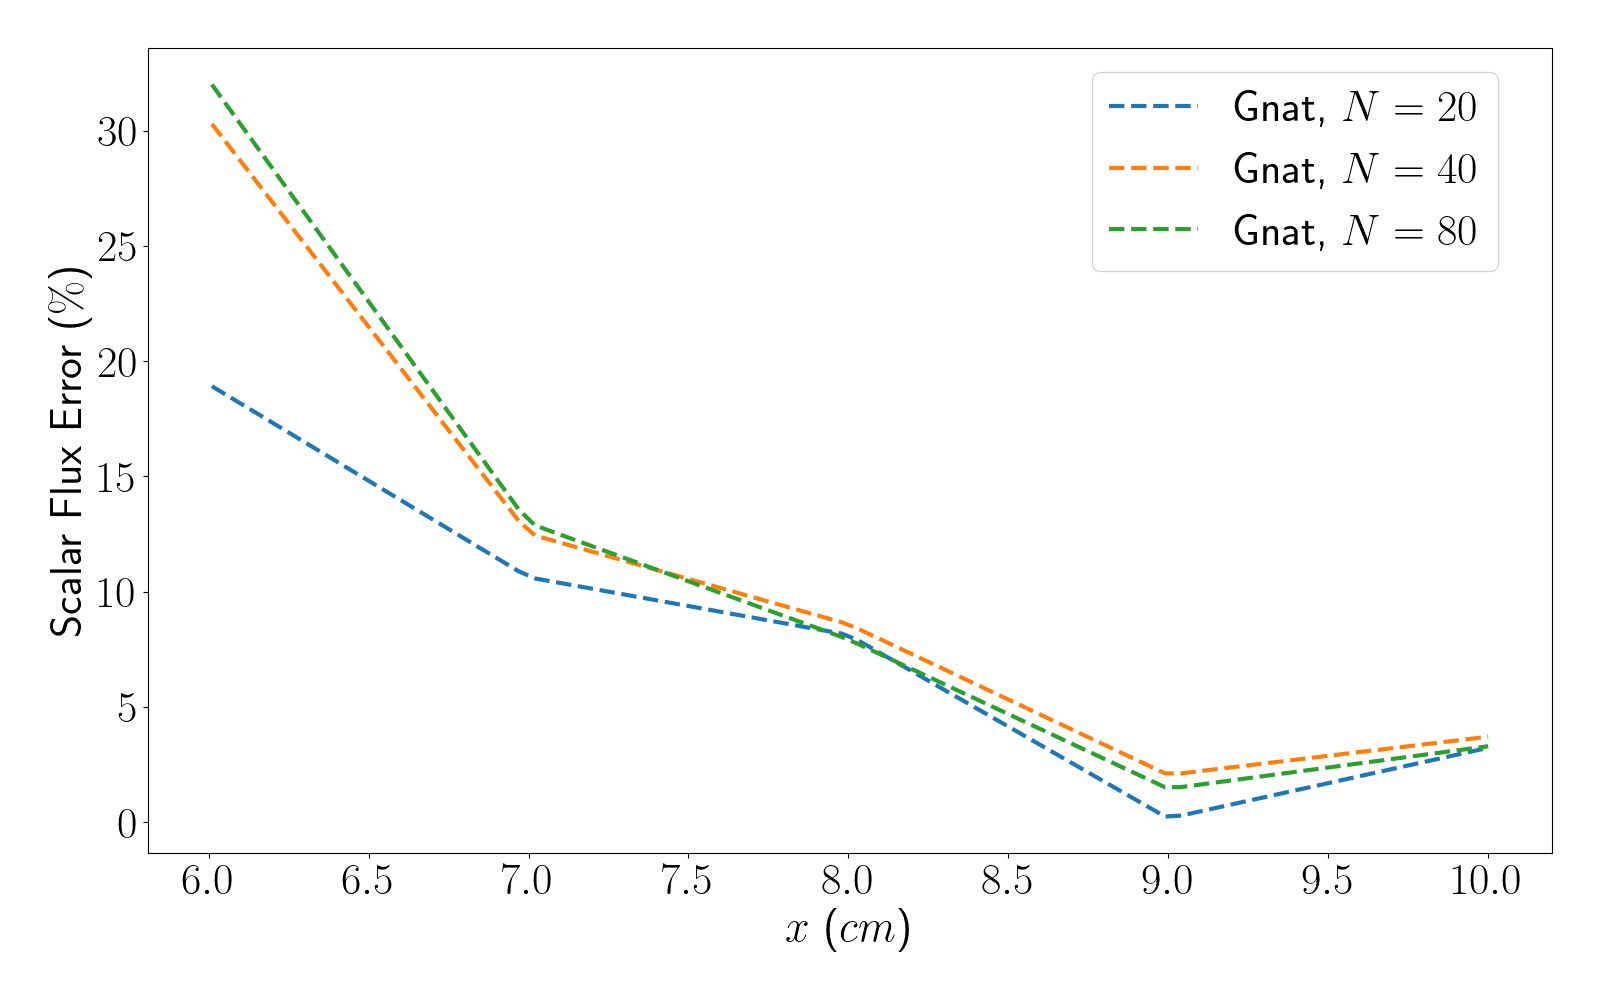
\includegraphics[width=\textwidth]{images/verification/1d_slab/1D_analytical_flux_error_1.png}
        \caption{Relative error in the numerical scalar flux.}
        \label{fig:verification:1D_flux:10_elem_error}
    \end{subfigure}
    \caption{Comparison of the numerical and analytical scalar fluxes for a 10 element mesh.}
    \label{fig:verification:1D_flux_10_elem}
\end{figure}
\begin{figure}[H]
    \centering
    %\hfill
    \begin{subfigure}[b]{0.495\textwidth}
        \centering
        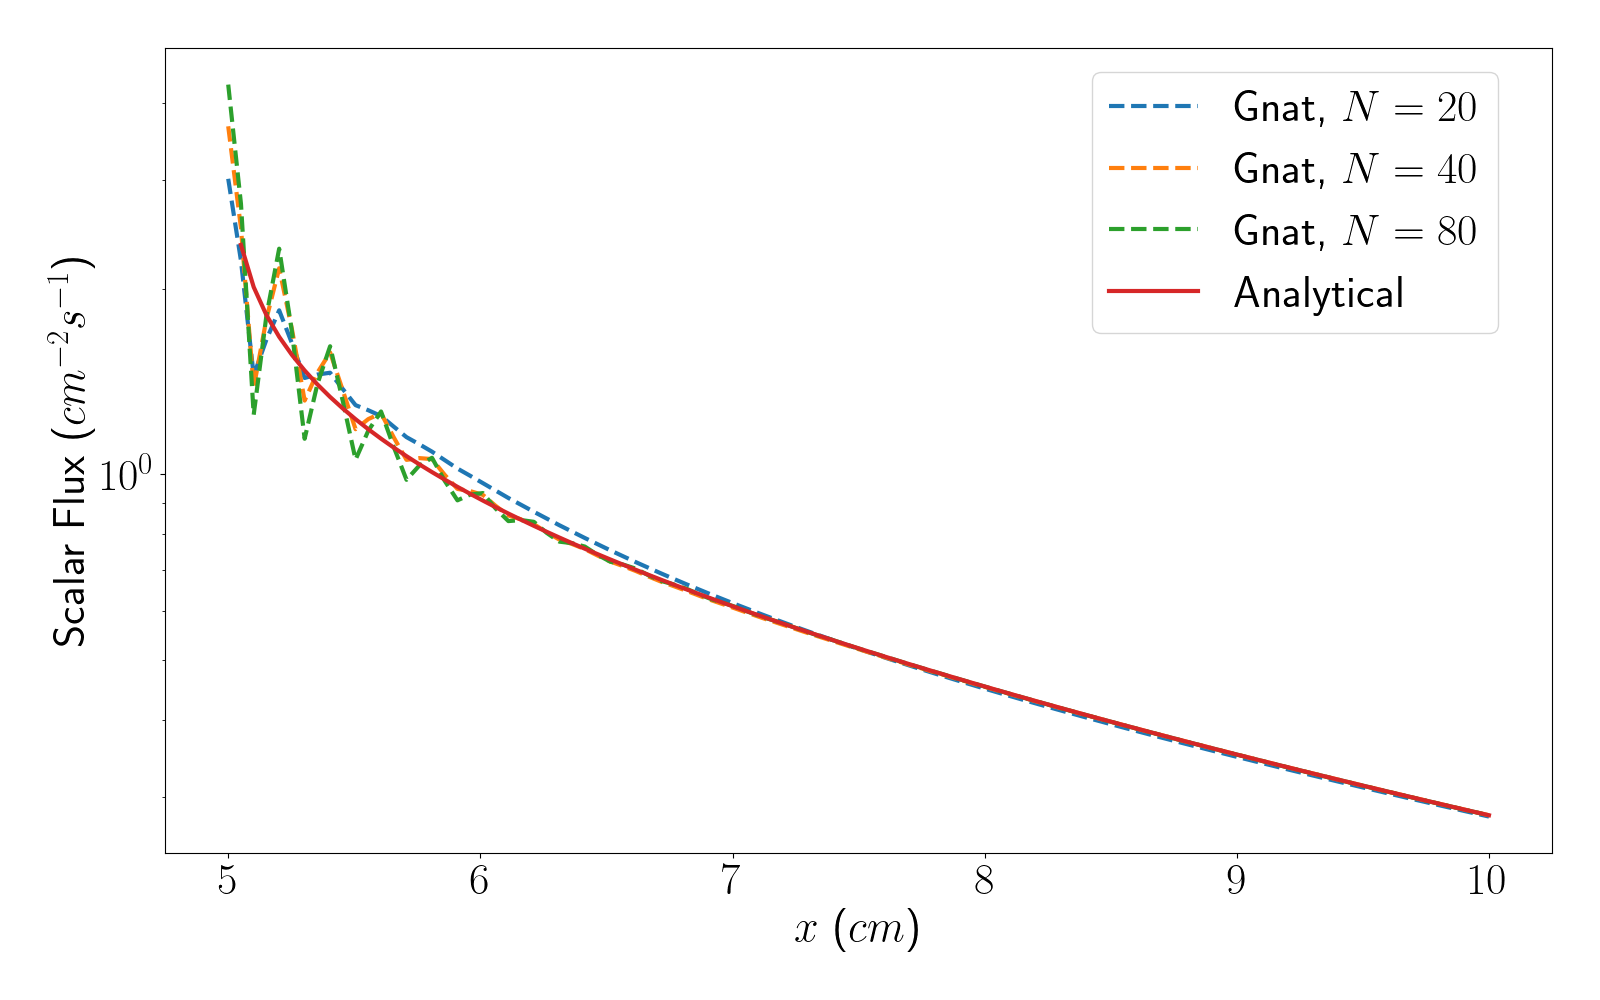
\includegraphics[width=\textwidth]{images/verification/1d_slab/1D_analytical_flux_2.png}
        \caption{Numerical and analytical scalar fluxes.}
        \label{fig:verification:1D_flux:100_elem}
    \end{subfigure}
    \hfill
    \begin{subfigure}[b]{0.495\textwidth}
        \centering
        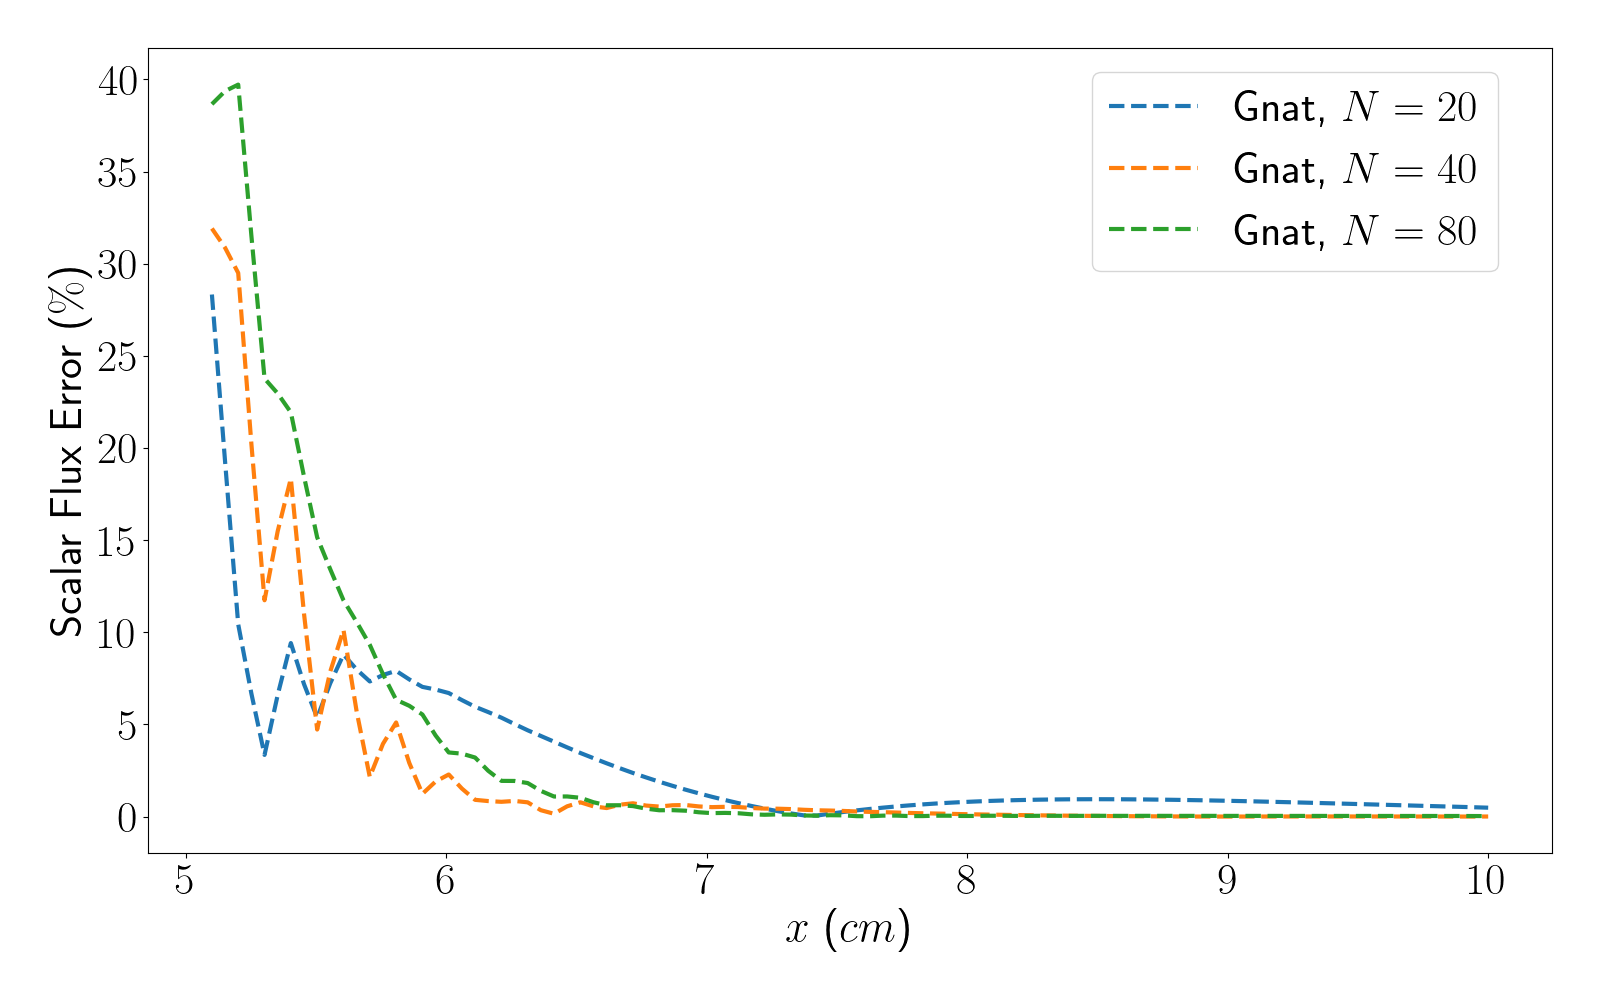
\includegraphics[width=\textwidth]{images/verification/1d_slab/1D_analytical_flux_error_2.png}
        \caption{Relative error in the numerical scalar flux.}
        \label{fig:verification:1D_flux:100_elem_error}
    \end{subfigure}
    \caption{Comparison of the numerical and analytical scalar fluxes for a 100 element mesh.}
    \label{fig:verification:1D_flux_100_elem}
\end{figure}
\begin{figure}[H]
    \centering
    %\hfill
    \begin{subfigure}[b]{0.495\textwidth}
        \centering
        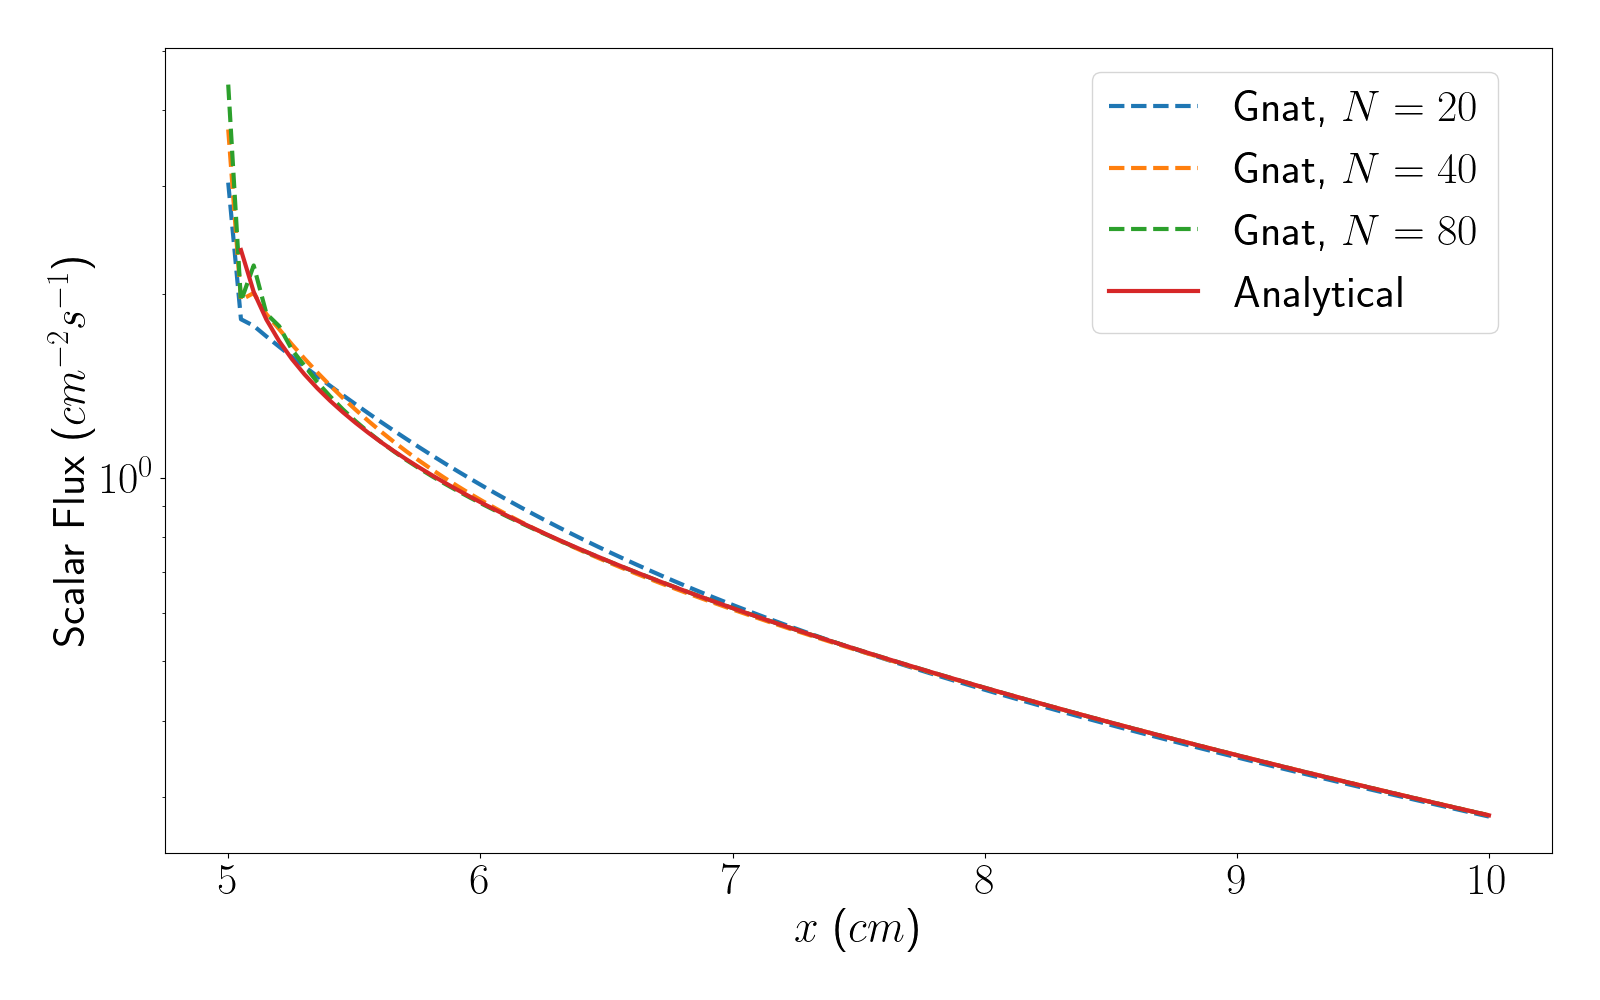
\includegraphics[width=\textwidth]{images/verification/1d_slab/1D_analytical_flux_3.png}
        \caption{Numerical and analytical scalar fluxes.}
        \label{fig:verification:1D_flux:1000_elem}
    \end{subfigure}
    \hfill
    \begin{subfigure}[b]{0.495\textwidth}
        \centering
        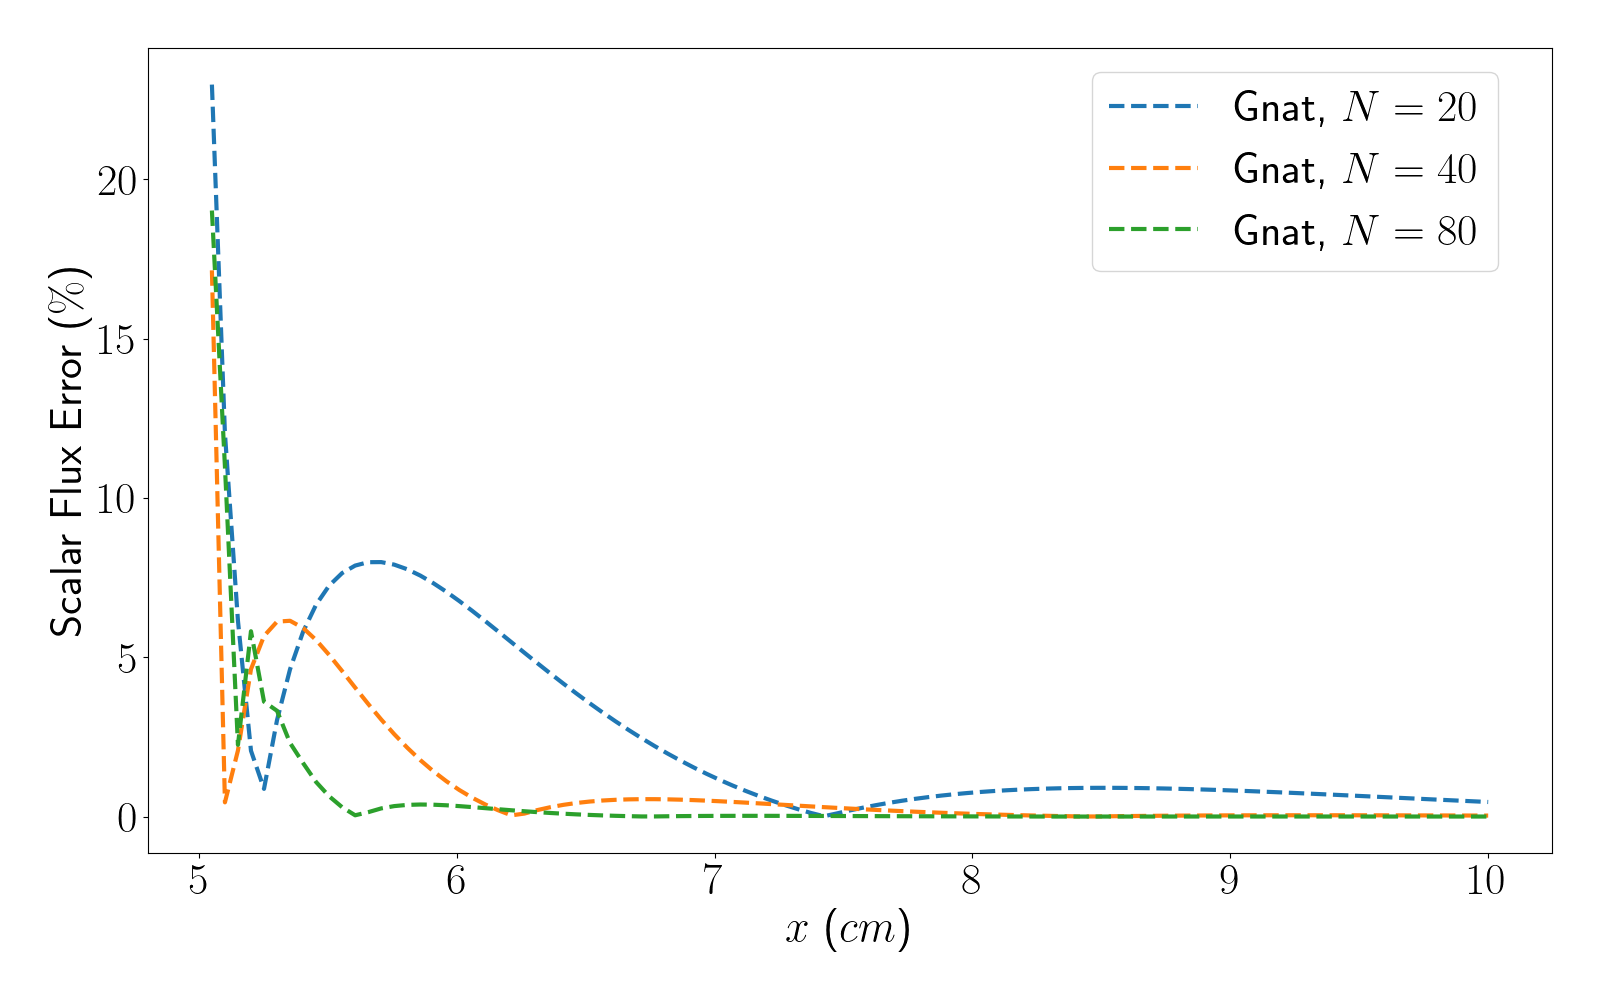
\includegraphics[width=\textwidth]{images/verification/1d_slab/1D_analytical_flux_error_3.png}
        \caption{Relative error in the numerical scalar flux.}
        \label{fig:verification:1D_flux:1000_elem_error}
    \end{subfigure}
    \caption{Comparison of the numerical and analytical scalar fluxes for a 1000 element mesh.}
    \label{fig:verification:1D_flux_1000_elem}
\end{figure}

In the extremely coarse mesh case where only 10 elements are used (Figure~\ref{fig:verification:1D_flux_10_elem}); the numerical scalar fluxes oscillate about the analytical solution by a wide margin with absolute relative errors of up to 30\%. The numerical solution entirely fails to represent the analytical scalar flux at $x = 5$ cm. Refinement in the angular domain does not result in an increase in accuracy for these coarse mesh results; the additional angular directions only serve to further increase the scalar flux error near the source. However, the scalar flux error decreases as the fluxes move further away from the slab source indicating that this localized heterogeneity is responsible for the instability of the numerical fluxes. Moving to 100 elements (Figure~\ref{fig:verification:1D_flux_100_elem}), the numerical solutions begin to capture the analytical solution closer to the slab source and additional angular refinement results in improvements in the prediction of the analytical solution further downwind from $x = 5$ cm. The peak error rises to 40\% near the source, which is likely caused by the singularity previously discussed. At the final refinement of 1000 elements, the angular resolution of the problem starts to dominate the error in the numerical solution. The low order quadrature set with 10 directions per octant overshoots the analytical solution. Refining the angular quadrature to 40 directions per octant results in a decrease in the relative error to near-zero everywhere with the exception of the neighborhood near the slab source. The convergence to the analytical solution as the angular domain is refined lends credibility to the implementation of the \acrshort{sn} transport solver.

\subsection{The Kobayashi Benchmarks}
\label{verification:radiation_transport_sn:kobayashi}

The next series of verification problems are the Kobayashi benchmark problems \cite{kobayashi_benchmarks}. These have become a series of standard transport benchmarks due to the presence of a large void regions and several order of magnitude jump discontinuities in cross section, which are challenging for second order transport methods (such as the \acrshort{saaf} method) to resolve. These large void regions are also set up such that they result in long streaming paths and deep penetrations, which are challenging for the \acrshort{sn} method to accurately predict due to ray effects. There are six benchmark problems in the Kobayashi suite: three problems that use pure absorbers and three problems that use a scattering ratio of $\Sigma_{s} / \Sigma_{t} = 0.5$. This work elects to verify the \acrshort{sn} radiation transport solver with the scattering cases to test as many capabilities of the solver in 3D as possible. All of the benchmark problems use the material properties in Table~\ref{table:kobayashi_props} \cite{kobayashi_benchmarks}. The volumetric particle source and the scattering cross sections are isotropic.
\begin{table}[H]
    \centering
    \singlespacing
    \caption[Material properties for the Kobayashi benchmark problems.]{Material properties for the Kobayashi benchmark problems. Adapted from Kobayashi and Sugimura \cite{kobayashi_benchmarks}.}
    \begin{tabular}{|cccc|}
        \hline
        \textbf{Region} & \makecell{$Q^{\text{ext}}$ \\ cm\textsuperscript{-3} s\textsuperscript{-1}} & \makecell{$\Sigma_{t}$ \\ cm\textsuperscript{-1}}  & \makecell{$\Sigma_{s}$ \\ cm\textsuperscript{-1}} \\
        \hline
        1 & $1.0$ & $1\times10^{-1}$ & $5\times 10^{-2}$\\
        2 & $0.0$ & $1\times10^{-4}$ & $5\times 10^{-5}$\\
        3 & $0.0$ & $1\times10^{-1}$ & $5\times 10^{-2}$\\
        \hline
    \end{tabular}
    \label{table:kobayashi_props}
\end{table}

The first of these benchmark problems is a square particle source embedded in a voided regions, which is then surrounded by a shield. Reflective boundary conditions are applied along the x-z plane ($y = 0\text{ cm}$), x-y plane ($z = 0\text{ cm}$) and y-z plane ($x = 0\text{ cm}$). Vacuum boundary conditions are applied along the x-z plane ($y = 100\text{ cm}$), x-y plane ($z = 100\text{ cm}$) and y-z plane ($x = 100\text{ cm}$). The geometry of the first benchmark problem can be found in Figure~\ref{fig:verification:sn_kobayashi_1_geo}. The second benchmark problem is a square particle source embedded in a shield. There is a straight voided duct penetrating this shield, starting from the particle source and moving through the domain until it reaches a vacuum boundary. Reflective boundary conditions are applied along the x-z plane ($y = 0\text{ cm}$), x-y plane ($z = 0\text{ cm}$) and y-z plane ($x = 0\text{ cm}$). Vacuum boundary conditions are applied along the x-z plane ($y = 100\text{ cm}$), x-y plane ($z = 60\text{ cm}$) and y-z plane ($x = 60\text{ cm}$). The geometry of this benchmark problem can be found in Figure~\ref{fig:verification:sn_kobayashi_2_geo}.
\begin{figure}[H]
    \centering
    \begin{subfigure}[b]{0.45\textwidth}
        \centering
        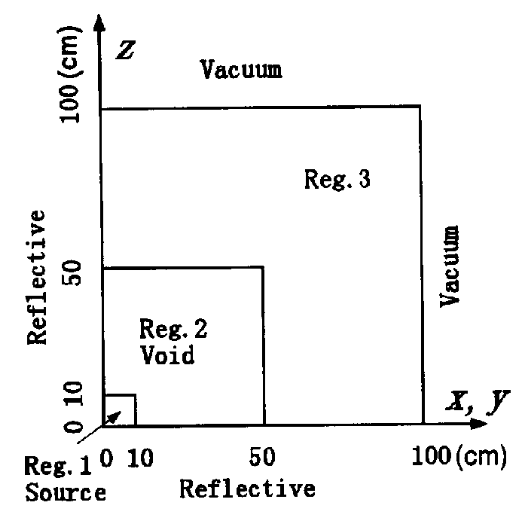
\includegraphics[width=\textwidth]{images/verification/sn_kobayashi/geometry/1_geo_1.png}
        \caption{x-y / y-z plane for the first Kobayashi problem.}
        \label{fig:verification:sn_kobayashi_1_geo:1}
    \end{subfigure}
    \hfill
    \begin{subfigure}[b]{0.45\textwidth}
        \centering
        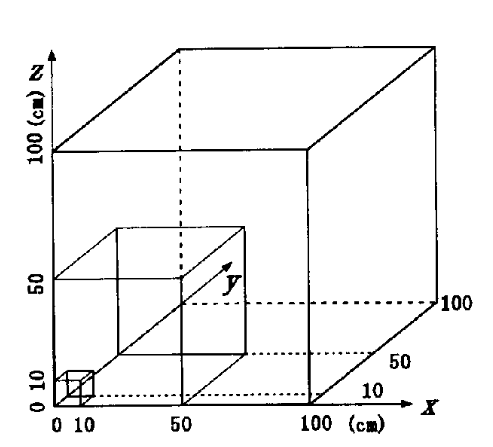
\includegraphics[width=\textwidth]{images/verification/sn_kobayashi/geometry/1_geo_2.png}
        \caption{Sketch of the first problem.}
        \label{fig:verification:sn_kobayashi_1_geo:2}
    \end{subfigure}
    \caption[Geometry for the first Kobayashi problem.]{Geometry for the first Kobayashi problem. Taken from Kobayashi and Sugimura \cite{kobayashi_benchmarks}.}
    \label{fig:verification:sn_kobayashi_1_geo}
\end{figure}
\begin{figure}[H]
    \centering
    \begin{subfigure}[b]{0.45\textwidth}
        \centering
        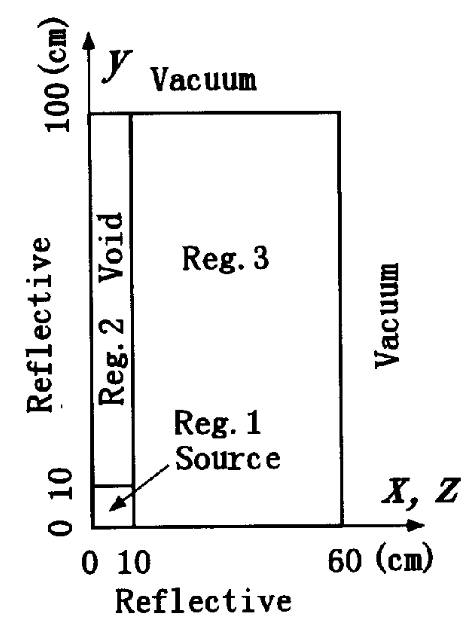
\includegraphics[width=\textwidth]{images/verification/sn_kobayashi/geometry/2_geo_1.png}
        \caption{x-y / y-z plane for the second Kobayashi problem.}
        \label{fig:verification:sn_kobayashi_2_geo:1}
    \end{subfigure}
    \hfill
    \begin{subfigure}[b]{0.45\textwidth}
        \centering
        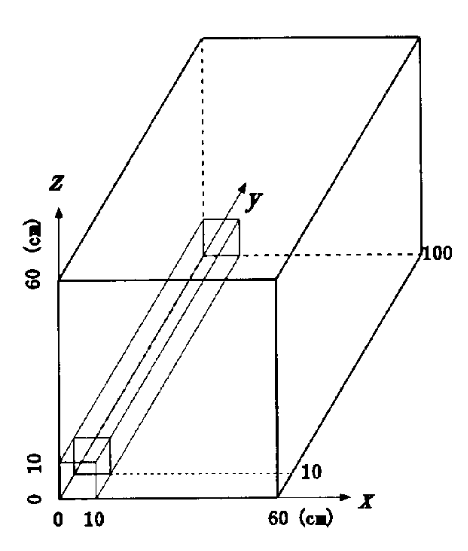
\includegraphics[width=\textwidth]{images/verification/sn_kobayashi/geometry/2_geo_2.png}
        \caption{Sketch of the second problem.}
        \label{fig:verification:sn_kobayashi_2_geo:2}
    \end{subfigure}
    \caption[Geometry for the second Kobayashi problem.]{Geometry for the second Kobayashi problem. Taken from Kobayashi and Sugimura \cite{kobayashi_benchmarks}.}
    \label{fig:verification:sn_kobayashi_2_geo}
\end{figure}
The third benchmark problem is a square particle source embedded in a shield. There is a voided duct penetrating the shielded region, starting at the particle source, taking three right angle turns, and exiting the domain at a vacuum boundary. Similar to the previous benchmark problems, reflective boundary conditions are applied along the x-z plane ($y = 0\text{ cm}$), x-y plane ($z = 0\text{ cm}$) and y-z plane ($x = 0\text{ cm}$). Vacuum boundary conditions are applied along the x-z plane ($y = 100\text{ cm}$), x-y plane ($z = 60\text{ cm}$) and y-z plane ($x = 60\text{ cm}$). The benchmark geometry for this dog-legged duct can be found in Figure~\ref{fig:verification:sn_kobayashi_3_geo}.
\begin{figure}[H]
    \centering
    \begin{subfigure}[b]{0.45\textwidth}
        \centering
        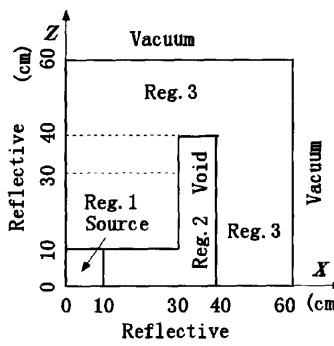
\includegraphics[width=\textwidth]{images/verification/sn_kobayashi/geometry/3_geo_1.png}
        \caption{x-z plane for the third Kobayashi problem.}
        \label{fig:verification:sn_kobayashi_3_geo:1}
    \end{subfigure}
    \hfill
    \begin{subfigure}[b]{0.45\textwidth}
        \centering
        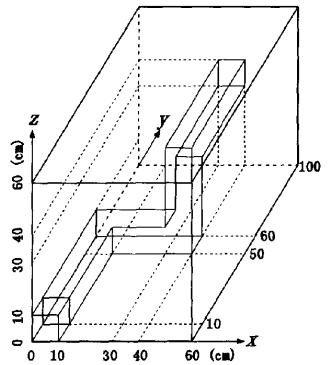
\includegraphics[width=\textwidth]{images/verification/sn_kobayashi/geometry/3_geo_2.png}
        \caption{Sketch of the third problem.}
        \label{fig:verification:sn_kobayashi_3_geo:2}
    \end{subfigure}
    \caption[Geometry for the third Kobayashi problem.]{Geometry for the third Kobayashi problem. Taken from Kobayashi and Sugimura \cite{kobayashi_benchmarks}.}
    \label{fig:verification:sn_kobayashi_3_geo}
\end{figure}

Numerical solutions to these three benchmark problems were conducted before the reflective boundary condition implementation in \acrshort{gnat} was complete. The mesh for the problem was unfolded across the x-z ($y = 0\text{ cm}$), x-y ($z = 0\text{ cm}$) and y-z ($x = 0\text{ cm}$) planes. This increases the size of the problem and places the source at the center of the domain to compensate for this deficiency. Each benchmark problem was meshed using uniform quadrilateral elements with side lengths of $5$ cm. This resulted in 72,000 elements in the first benchmark, 25,920 elements in the second problem, and 23,040 elements in the third problem. The finite element basis functions used were linear Lagrange functions. All benchmark cases used the \acrshort{pjfnk} solver with preconditioning provided by the hypre package BoomerAMG and 30 \acrfull{gmres} vectors. All benchmark problems are solved with a Gauss-Chebyshev angular quadrature set. The first benchmark problem used 10 polar angles and 10 azimuthal angles per octant of the unit sphere, resulting in a total of 800 angular directions. The second and third benchmark problems used 16 azimuthal angles and 12 polar angles per octant of the unit sphere for a total of 1536 angular directions. An initial residual vector magnitude of $3.339351\times 10^{3}$ was obtained for the first problem, which was the largest across each of the Kobayashi benchmarks. This led to the use of a relative convergence criteria of $10^{-12}$ to ensure that the magnitude of the final residual vector was below $10^{-8}$ on convergence. Experimentation with a reduced order angular quadrature showed that any additional refinement of the relative convergence criteria did not result in any substantial changes to the result of the Kobayashi problems.

\begin{figure}[H]
    \centering
    \begin{subfigure}[b]{0.4\textwidth}
        \centering
        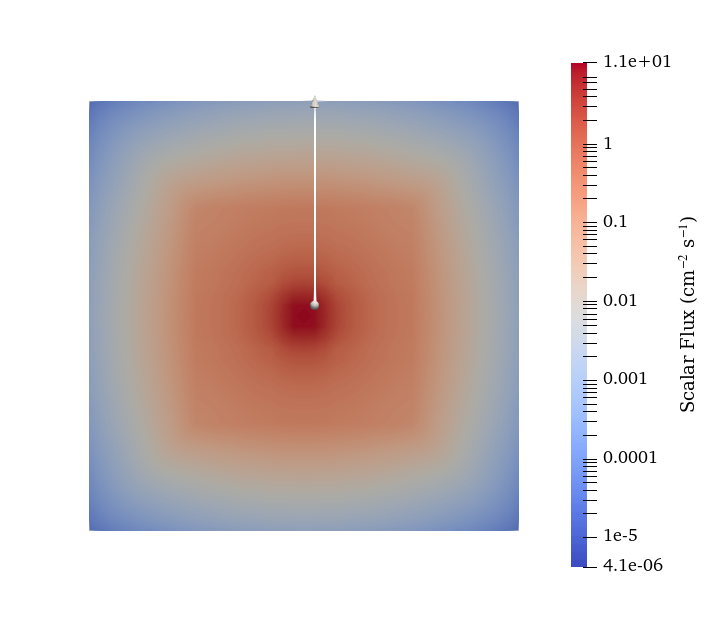
\includegraphics[width=\textwidth]{images/verification/sn_kobayashi/1/kobayashi_1a_flux_map.png}
        \caption{Scalar flux distribution associated with the line plot. The cutting plane is the x-y plane at $z = 5\text{ cm}$.}
        \label{fig:verification:sn_kobayashi_1a:flux}
    \end{subfigure}
    \hfill
    \begin{subfigure}[b]{0.59\textwidth}
        \centering
        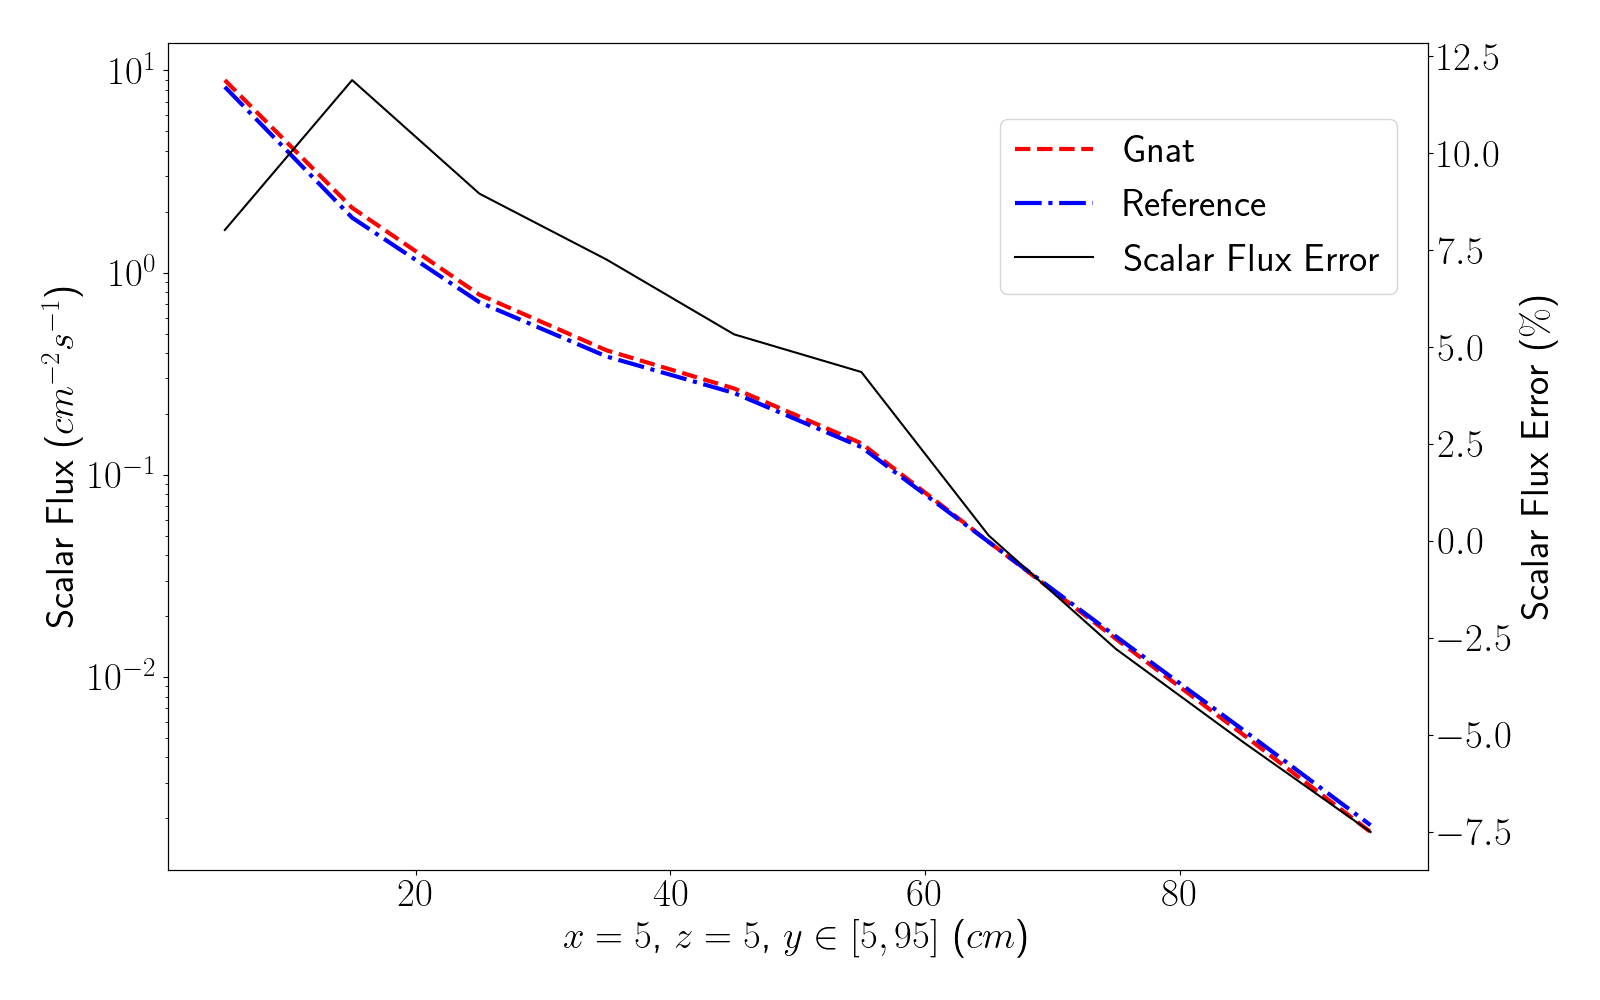
\includegraphics[width=\textwidth]{images/verification/sn_kobayashi/1/kobayashi_1a.png}
        \caption{Comparison with the benchmark problem. Reference taken from Kobayashi and Sugimura \cite{kobayashi_benchmarks}.}
        \label{fig:verification:sn_kobayashi_1a:line_plot}
    \end{subfigure}
    \caption{Results of the Kobayashi benchmark 1a.}
    \label{fig:verification:sn_kobayashi_1a}
\end{figure}

\begin{figure}[H]
    \centering
    \begin{subfigure}[b]{0.4\textwidth}
        \centering
        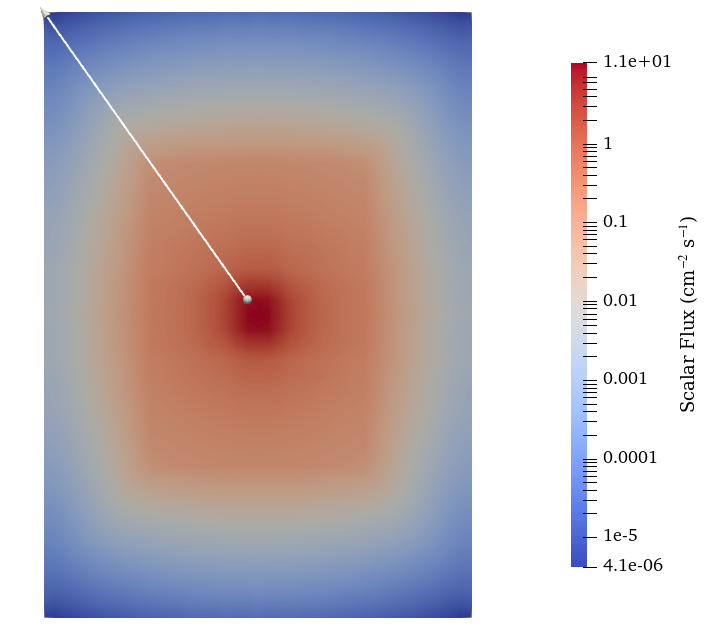
\includegraphics[width=\textwidth]{images/verification/sn_kobayashi/1/kobayashi_1b_flux_map.png}
        \caption{Scalar flux distribution associated with the line plot. The cutting plane has a normal vector of $\{-1/\sqrt{2}, -1/\sqrt{2}, 0\}$ and passes through the point $\{5\text{ cm}, 5\text{ cm}, 5\text{ cm}\}$.}
        \label{fig:verification:sn_kobayashi_1b:flux}
    \end{subfigure}
    \hfill
    \begin{subfigure}[b]{0.59\textwidth}
        \centering
        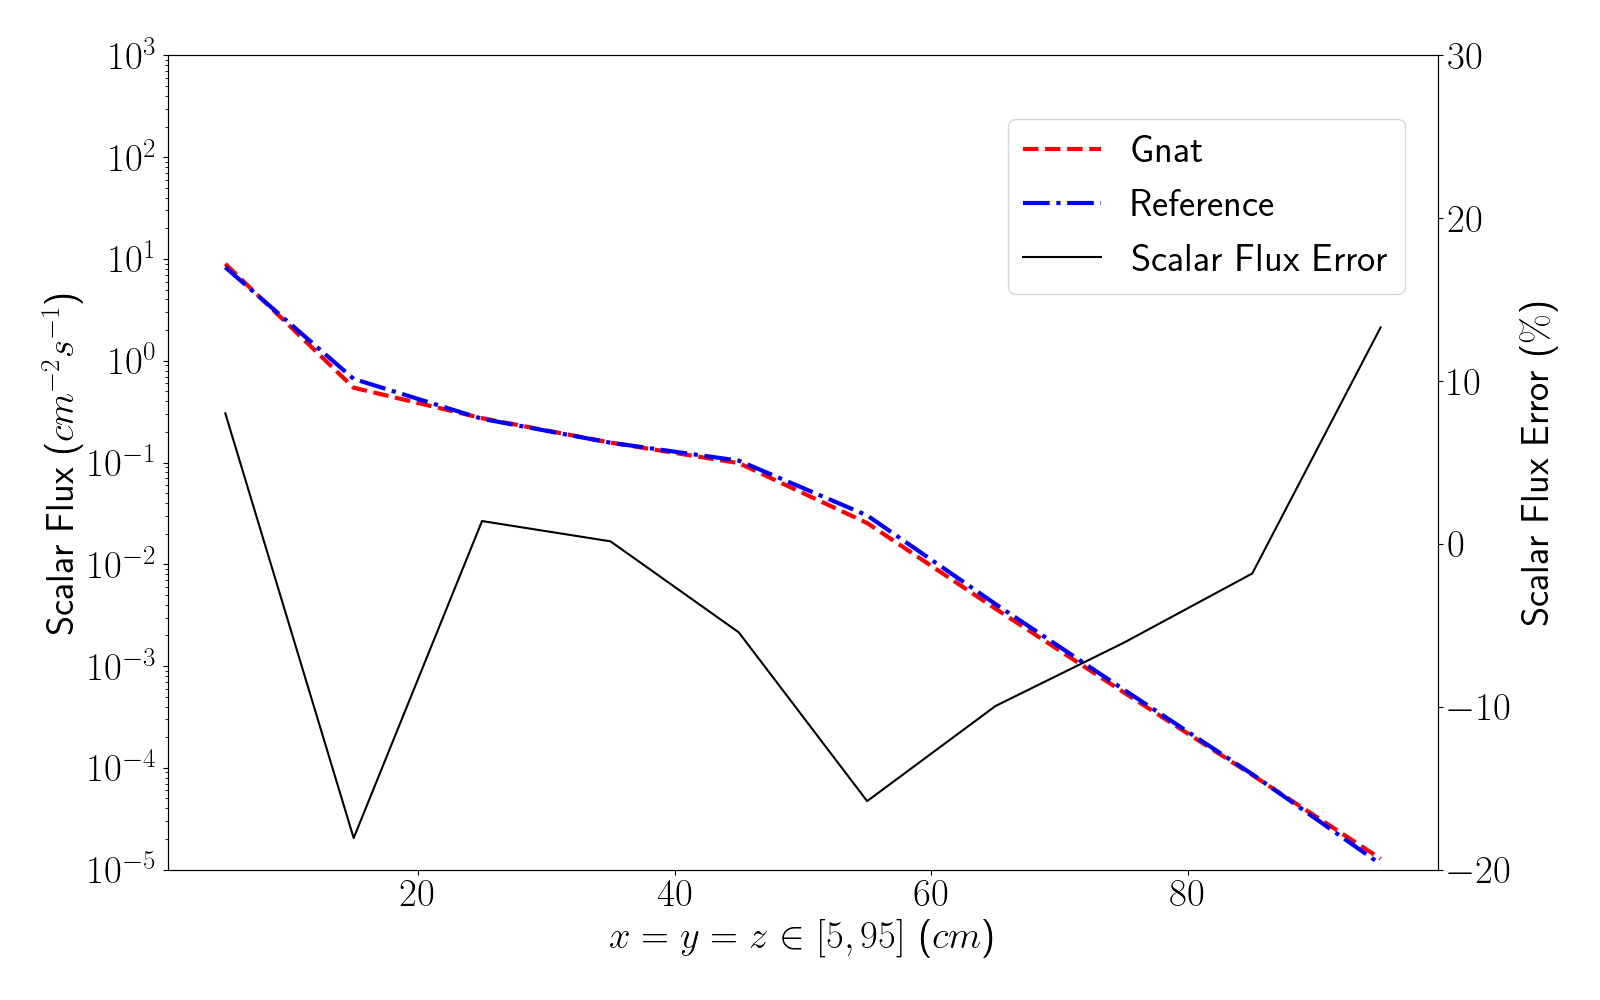
\includegraphics[width=\textwidth]{images/verification/sn_kobayashi/1/kobayashi_1b.png}
        \caption{Comparison with the benchmark problem. Reference taken from Kobayashi and Sugimura \cite{kobayashi_benchmarks}.}
        \label{fig:verification:sn_kobayashi_1b:line_plot}
    \end{subfigure}
    \caption{Results of the Kobayashi benchmark 1b.}
    \label{fig:verification:sn_kobayashi_1b}
\end{figure}

\begin{figure}[H]
    \centering
    \begin{subfigure}[b]{0.4\textwidth}
        \centering
        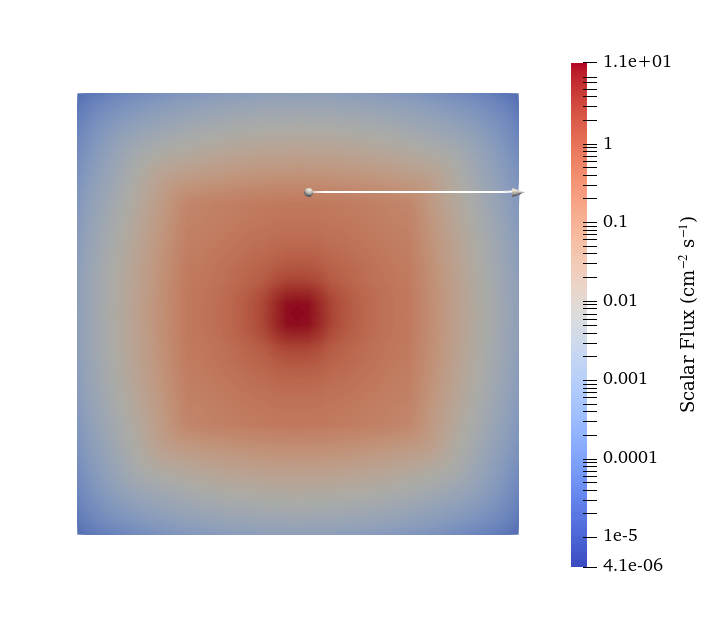
\includegraphics[width=\textwidth]{images/verification/sn_kobayashi/1/kobayashi_1c_flux_map.png}
        \caption{Scalar flux distribution associated with the line plot. The cutting plane is the x-y plane at $z = 5\text{ cm}$.}
        \label{fig:verification:sn_kobayashi_1c:flux}
    \end{subfigure}
    \hfill
    \begin{subfigure}[b]{0.59\textwidth}
        \centering
        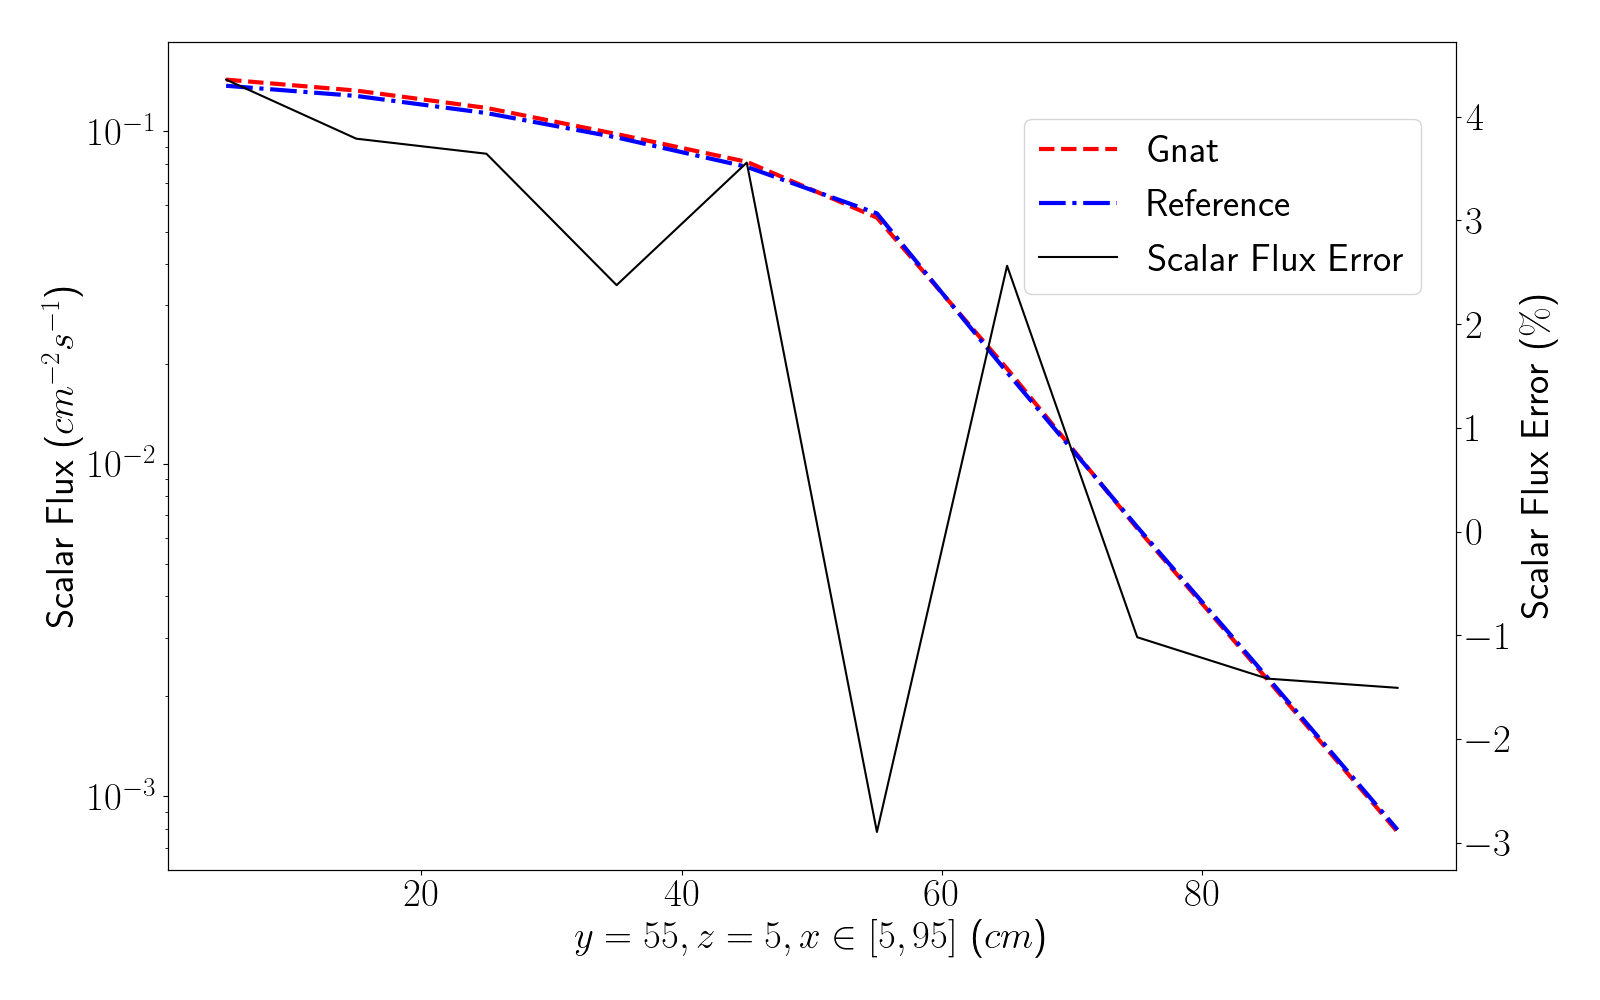
\includegraphics[width=\textwidth]{images/verification/sn_kobayashi/1/kobayashi_1c.png}
        \caption{Comparison with the benchmark problem. Reference taken from Kobayashi and Sugimura \cite{kobayashi_benchmarks}.}
        \label{fig:verification:sn_kobayashi_1c:line_plot}
    \end{subfigure}
    \caption{Results of the Kobayashi benchmark 1c.}
    \label{fig:verification:sn_kobayashi_1c}
\end{figure}

The results for the first benchmark problem can be found in Figures~\ref{fig:verification:sn_kobayashi_1a} to \ref{fig:verification:sn_kobayashi_1c} where they are compared with the solutions obtained by Kobayashi and Sugimura \cite{kobayashi_benchmarks}. In general, the results obtained with the \acrshort{sn} method using the \acrshort{saaf} spatial discretization agree well with the benchmark problem. In the case of Figure~\ref{fig:verification:sn_kobayashi_1a:line_plot} the relative scalar flux error reaches a maximum along the interface between the voided region and the particle source, which represents a large jump discontinuity in both cross section and the particle source. The uniform meshing scheme with the level of coarseness used is unable to capture that discontinuity, resulting in an over-prediction error. In the case of Figure~\ref{fig:verification:sn_kobayashi_1b:line_plot} this behavior is amplified by the point discontinuity at both the corner of the particle source and the interior corner of the shield, resulting in the two error peaks at 15 cm and 55 cm. The numerical scalar flux solution behaves quite well in the case of the lined plotted in Figure~\ref{fig:verification:sn_kobayashi_1c:line_plot} where the maximum error occurs at the corner of the shield. In general, the \acrshort{sn} solver proves to be capable of predicting the behavior of the first Kobayashi problem over the majority of the domain, with particularly good performance in regions that do not have large jump discontinuities in material properties or sources. 

The results for the second benchmark problem can be found in Figure~\ref{fig:verification:sn_kobayashi_2a} and Figure~\ref{fig:verification:sn_kobayashi_2b}. This duct problem is prone to ray effects when solved with \acrshort{sn} transport solvers due to the presence of a long streaming path moving from the localized particle source to the vacuum boundary. It can be seen that the error starts at 10\%, decreases, and then starts increasing over the plotted line in Figure~\ref{fig:verification:sn_kobayashi_2a:line_plot} until it reaches a maximum at 95 cm. This increase in error over the duct is caused by ray effects and the cross section discontinuity along the edge of the duct, which can be further visualized in Figure~\ref{fig:verification:sn_kobayashi_2b:line_plot}. The error in the numerical scalar flux starts at 40\% and drops to -40\% over the length of the duct. The scalar flux plotted through the diffuse region of the domain remains error-free by comparison. This indicates that not enough directions have been provided to properly resolve this deep penetration, especially when compared to the number of directions required to resolve the first benchmark problem.  
\begin{figure}[H]
    \centering
    \begin{subfigure}[b]{0.4\textwidth}
        \centering
        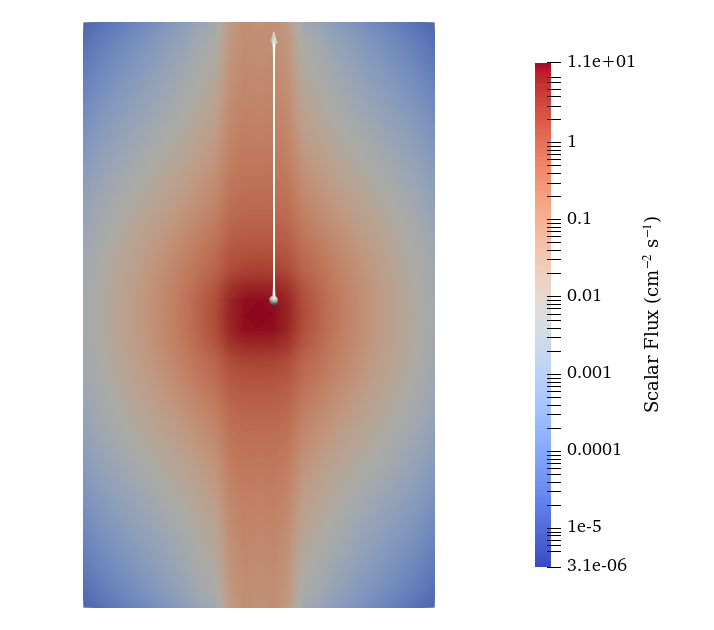
\includegraphics[width=\textwidth]{images/verification/sn_kobayashi/2/kobayashi_2a_flux_map.png}
        \caption{Scalar flux distribution associated with the line plot. The cutting plane is the x-y plane at $z = 5\text{ cm}$.}
        \label{fig:verification:sn_kobayashi_2a:flux}
    \end{subfigure}
    \hfill
    \begin{subfigure}[b]{0.59\textwidth}
        \centering
        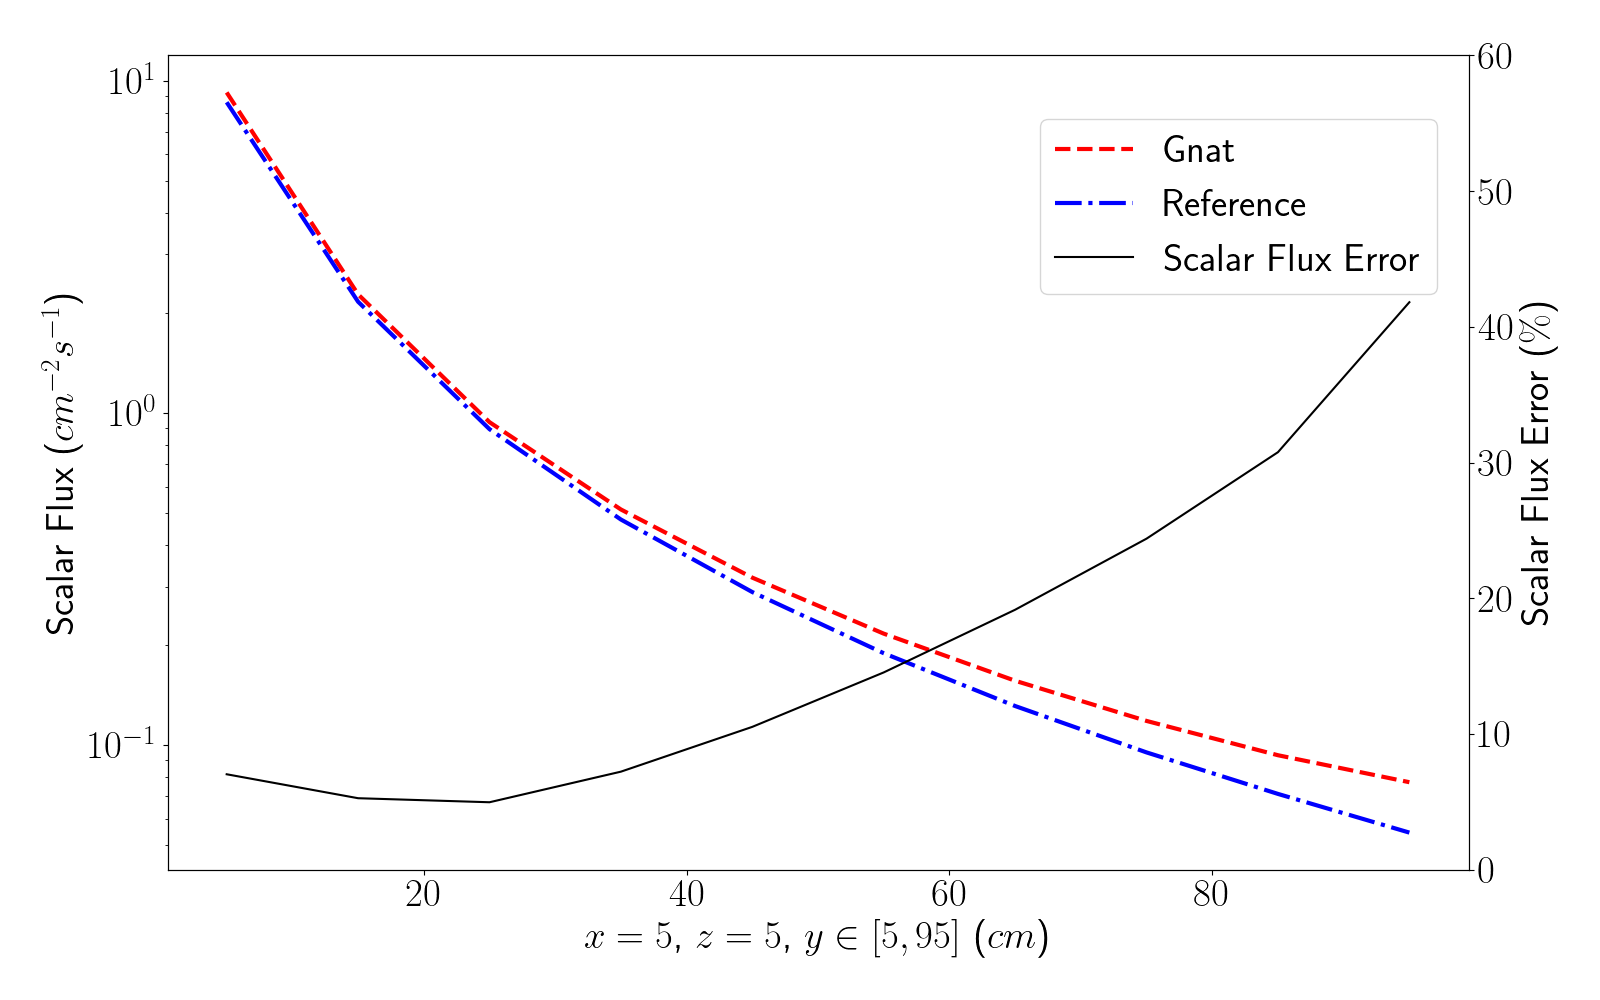
\includegraphics[width=\textwidth]{images/verification/sn_kobayashi/2/kobayashi_2a.png}
        \caption{Comparison with the benchmark problem. Reference taken from Kobayashi and Sugimura \cite{kobayashi_benchmarks}.}
        \label{fig:verification:sn_kobayashi_2a:line_plot}
    \end{subfigure}
    \caption{Results of the Kobayashi benchmark 2a.}
    \label{fig:verification:sn_kobayashi_2a}
\end{figure}

\begin{figure}[H]
    \centering
    \begin{subfigure}[b]{0.4\textwidth}
        \centering
        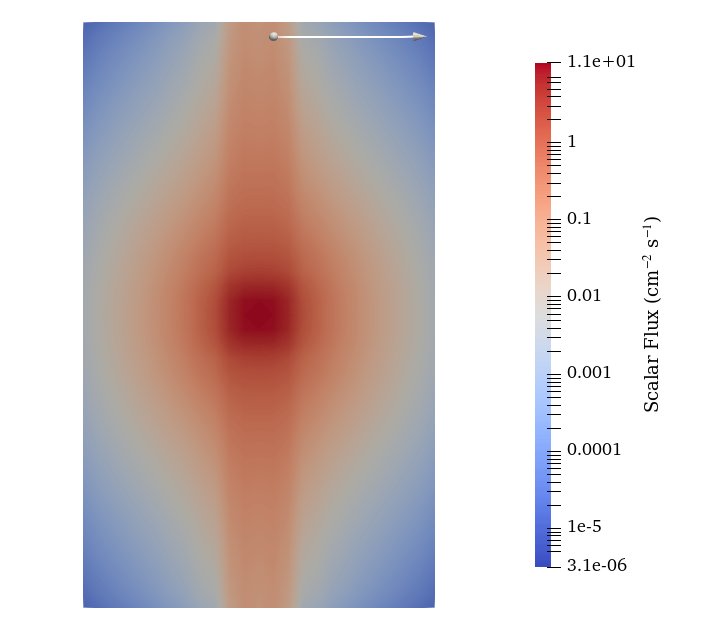
\includegraphics[width=\textwidth]{images/verification/sn_kobayashi/2/kobayashi_2b_flux_map.png}
        \caption{Scalar flux distribution associated with the line plot. The cutting plane is the x-y plane at $z = 5\text{ cm}$.}
        \label{fig:verification:sn_kobayashi_2b:flux}
    \end{subfigure}
    \hfill
    \begin{subfigure}[b]{0.59\textwidth}
        \centering
        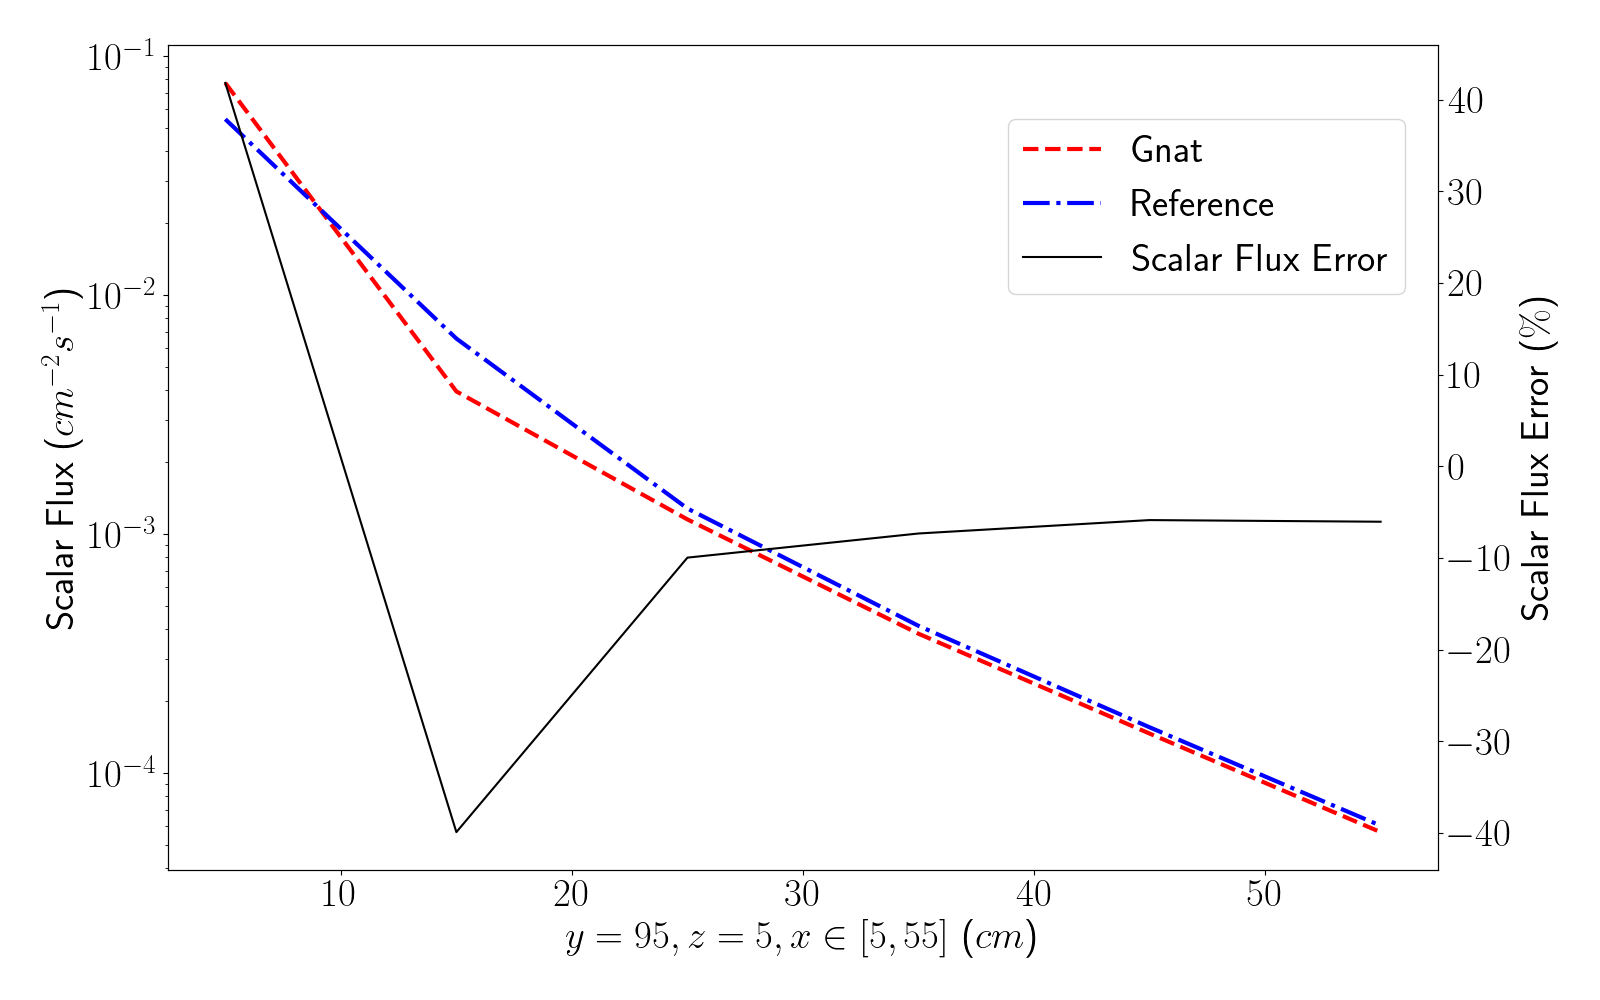
\includegraphics[width=\textwidth]{images/verification/sn_kobayashi/2/kobayashi_2b.png}
        \caption{Comparison with the benchmark problem. Reference taken from Kobayashi and Sugimura \cite{kobayashi_benchmarks}.}
        \label{fig:verification:sn_kobayashi_2b:line_plot}
    \end{subfigure}
    \caption{Results of the Kobayashi benchmark 2b.}
    \label{fig:verification:sn_kobayashi_2b}
\end{figure}

The results for the third benchmark problem can be found in Figures~\ref{fig:verification:sn_kobayashi_3a} to \ref{fig:verification:sn_kobayashi_3c}. This duct problem contains both a long streaming penetration which is prone to ray effects and several changes in the direction of the duct which requires scattering to be well resolved in the angular domain. Similar behavior to the second benchmark problem can be found in this third problem; Figure~\ref{fig:verification:sn_kobayashi_3a:line_plot} shows an increase in error along the duct due to an insufficiently resolved angular domain. This behavior changes as the scalar flux approaches the first turn in the duct; the error starts to decrease due to the influence of isotropic scattering from the shield, which the first straight-line segment of the duct terminates at. Plotting the scalar flux along the width of the duct in Figure~\ref{fig:verification:sn_kobayashi_3b:line_plot} shows a similar trend in error when compared the second benchmark (Figure~\ref{fig:verification:sn_kobayashi_2b:line_plot}). It is less severe in this case as the the line is closer to the volumetric source and scattering from the terminating shield aids in decreasing ray effects. Figure~\ref{fig:verification:sn_kobayashi_3c:line_plot} shows the scalar flux distribution within the duct after the three changes in direction. The scalar flux distribution is reasonably free of ray effects after the multiple scattering events required to pass through this deep penetration, and the most likely sources of error are the additional \acrshort{supg} stabilization added in the void region of the duct.

\begin{figure}[H]
    \centering
    \begin{subfigure}[b]{0.4\textwidth}
        \centering
        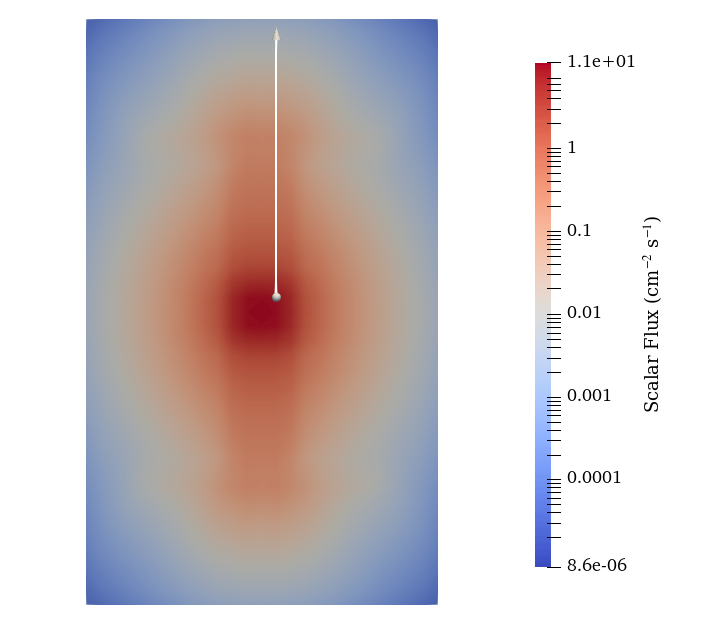
\includegraphics[width=\textwidth]{images/verification/sn_kobayashi/3/kobayashi_3a_flux_map.png}
        \caption{Scalar flux distribution associated with the line plot. The cutting plane is the x-y plane at $z = 5\text{ cm}$.}
        \label{fig:verification:sn_kobayashi_3a:flux}
    \end{subfigure}
    \hfill
    \begin{subfigure}[b]{0.59\textwidth}
        \centering
        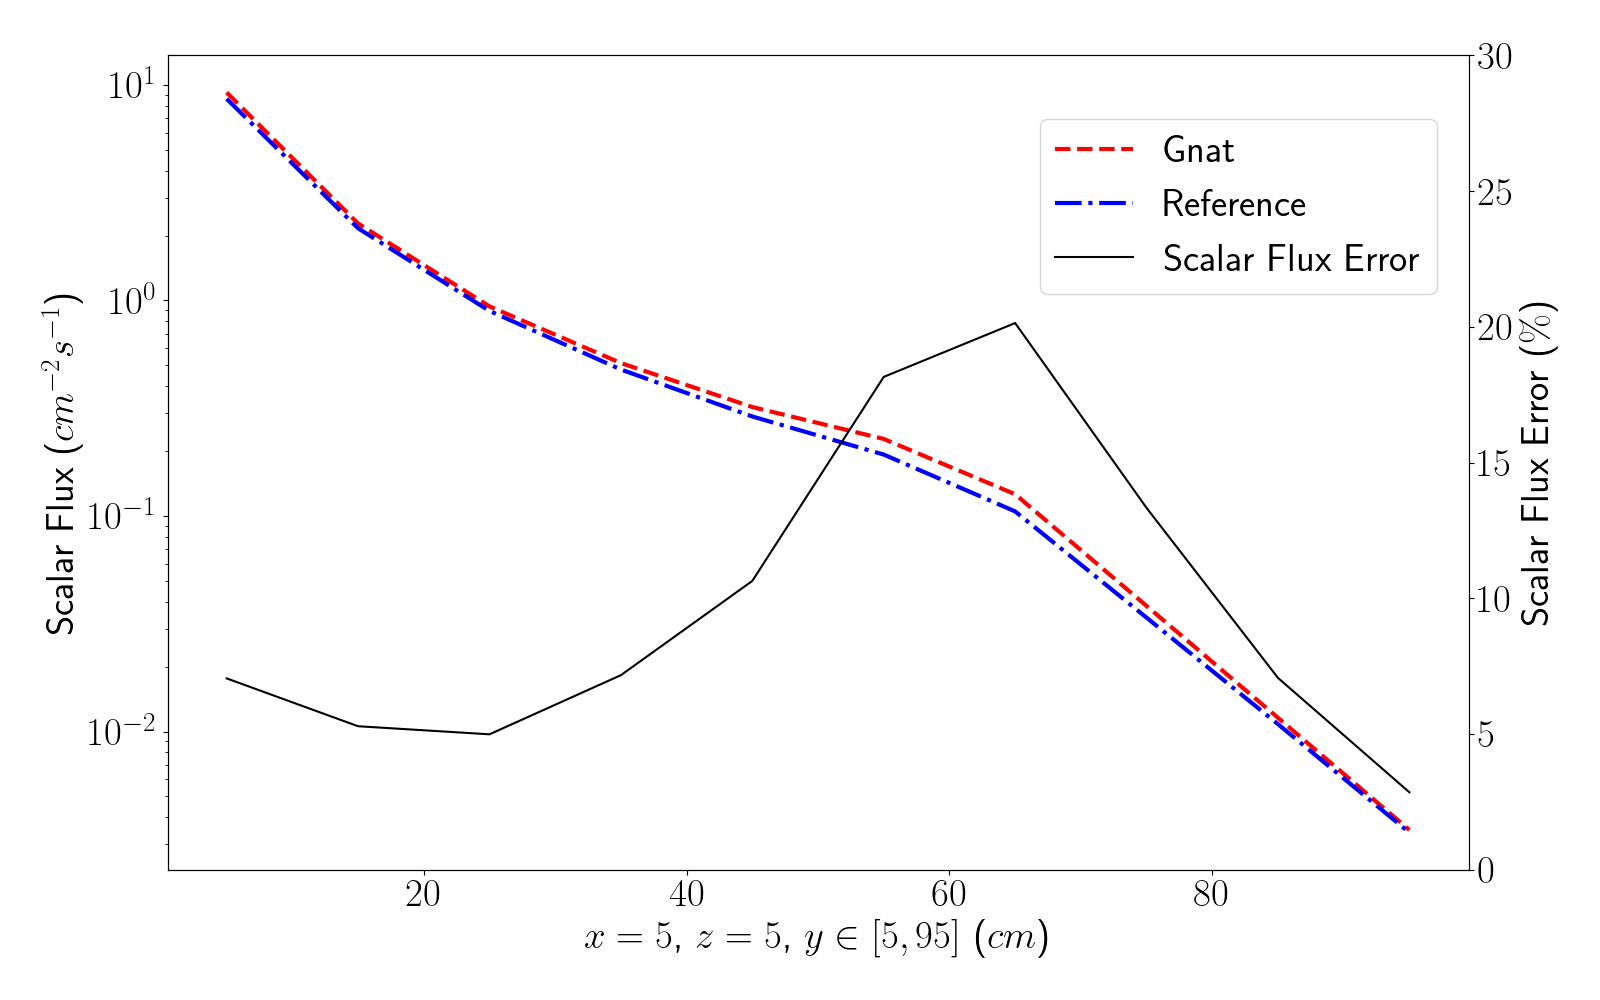
\includegraphics[width=\textwidth]{images/verification/sn_kobayashi/3/kobayashi_3a.png}
        \caption{Comparison with the benchmark problem. Reference taken from Kobayashi and Sugimura \cite{kobayashi_benchmarks}.}
        \label{fig:verification:sn_kobayashi_3a:line_plot}
    \end{subfigure}
    \caption{Results of the Kobayashi benchmark 3a.}
    \label{fig:verification:sn_kobayashi_3a}
\end{figure}

\begin{figure}[H]
    \centering
    \begin{subfigure}[b]{0.4\textwidth}
        \centering
        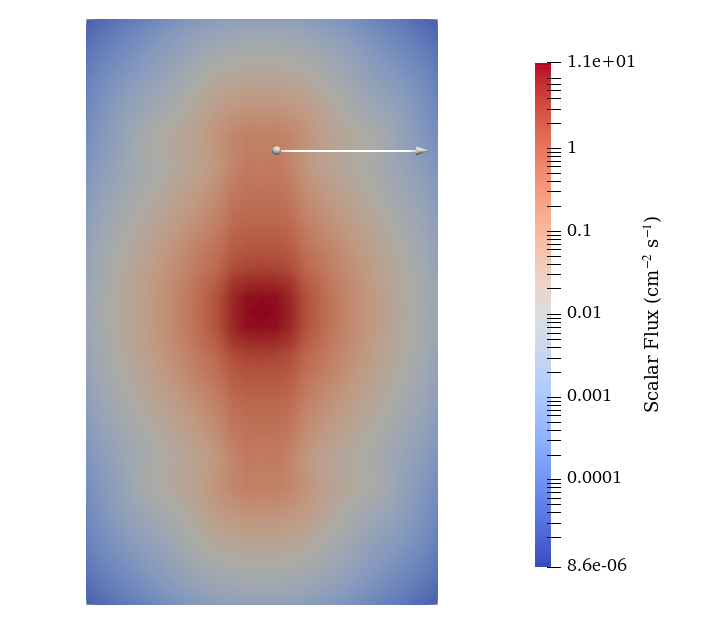
\includegraphics[width=\textwidth]{images/verification/sn_kobayashi/3/kobayashi_3b_flux_map.png}
        \caption{Scalar flux distribution associated with the line plot. The cutting plane is the x-y plane at $z = 5\text{ cm}$.}
        \label{fig:verification:sn_kobayashi_3b:flux}
    \end{subfigure}
    \hfill
    \begin{subfigure}[b]{0.59\textwidth}
        \centering
        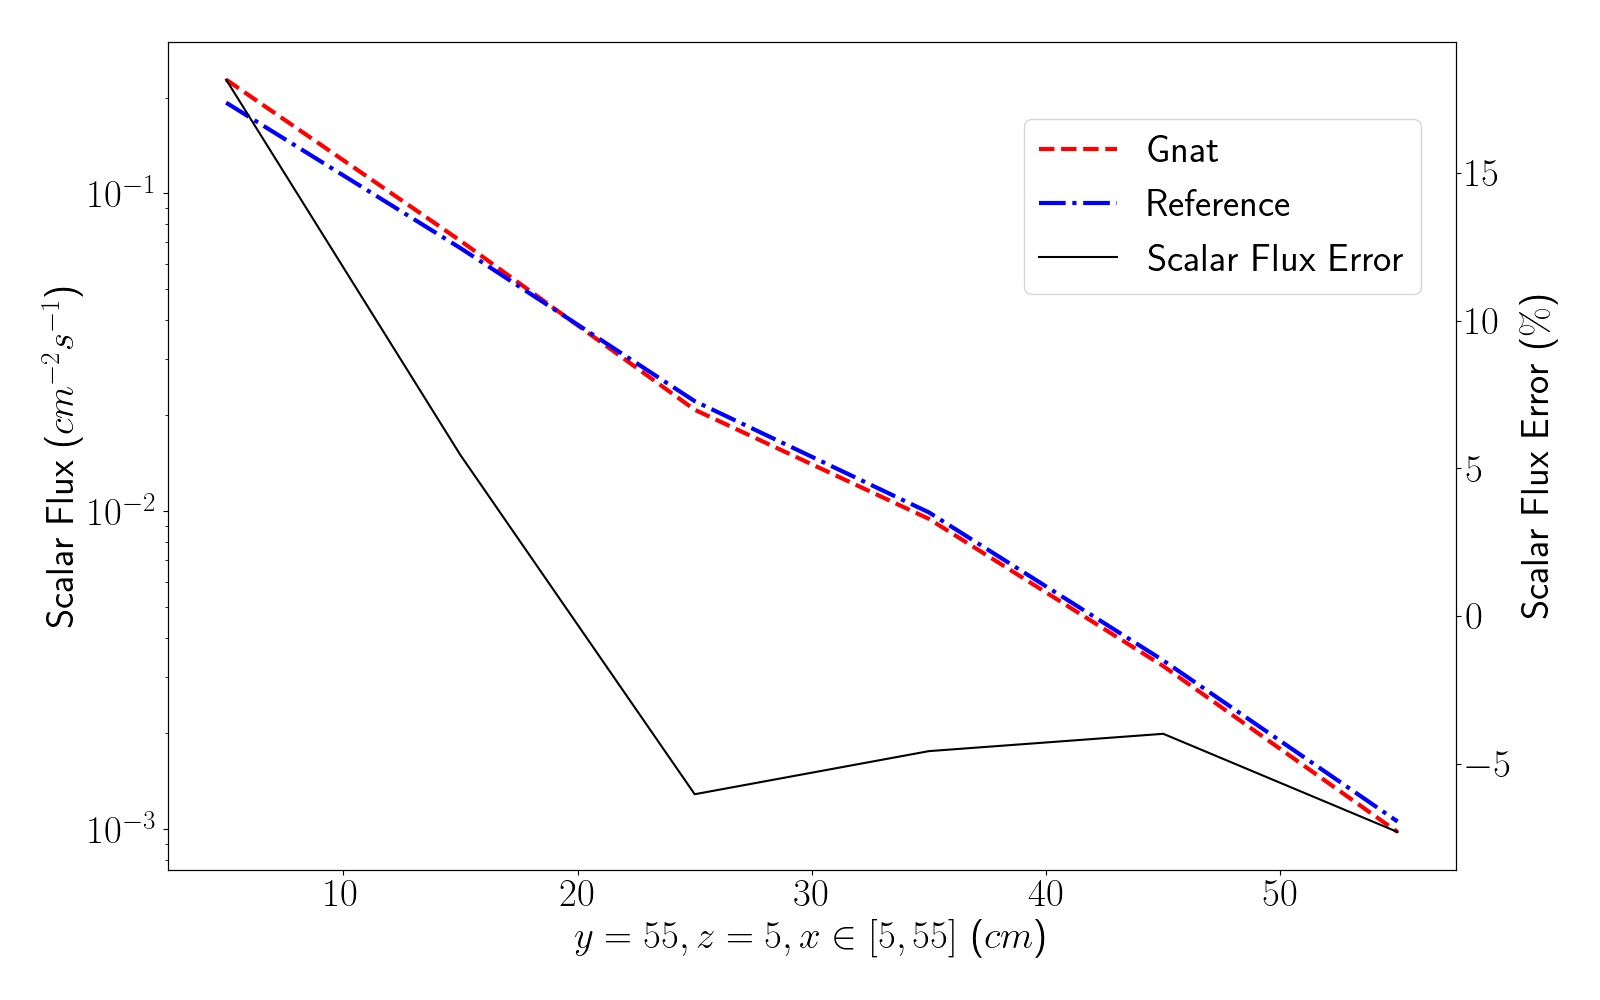
\includegraphics[width=\textwidth]{images/verification/sn_kobayashi/3/kobayashi_3b.png}
        \caption{Comparison with the benchmark problem. Reference taken from Kobayashi and Sugimura \cite{kobayashi_benchmarks}.}
        \label{fig:verification:sn_kobayashi_3b:line_plot}
    \end{subfigure}
    \caption{Results of the Kobayashi benchmark 3b.}
    \label{fig:verification:sn_kobayashi_3b}
\end{figure}

\begin{figure}[H]
    \centering
    \begin{subfigure}[b]{0.4\textwidth}
        \centering
        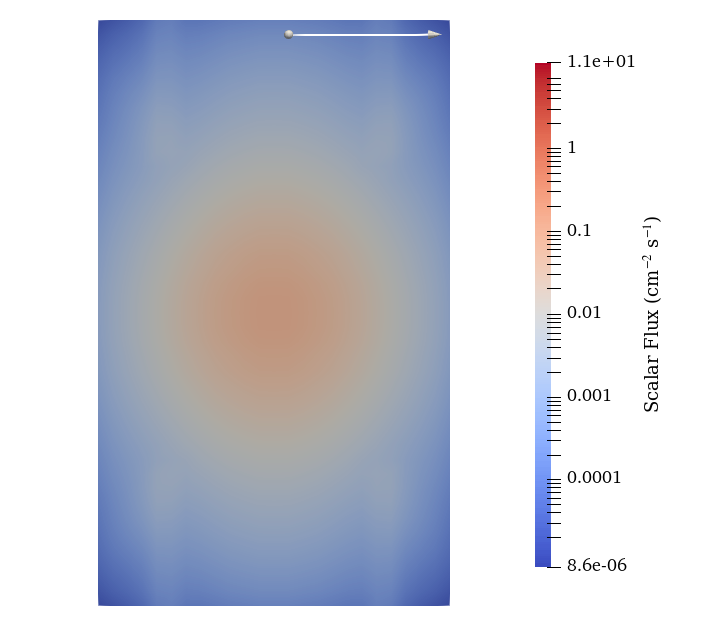
\includegraphics[width=\textwidth]{images/verification/sn_kobayashi/3/kobayashi_3c_flux_map.png}
        \caption{Scalar flux distribution associated with the line plot. The cutting plane is the x-y plane at $z = 35\text{ cm}$.}
        \label{fig:verification:sn_kobayashi_3c:flux}
    \end{subfigure}
    \hfill
    \begin{subfigure}[b]{0.59\textwidth}
        \centering
        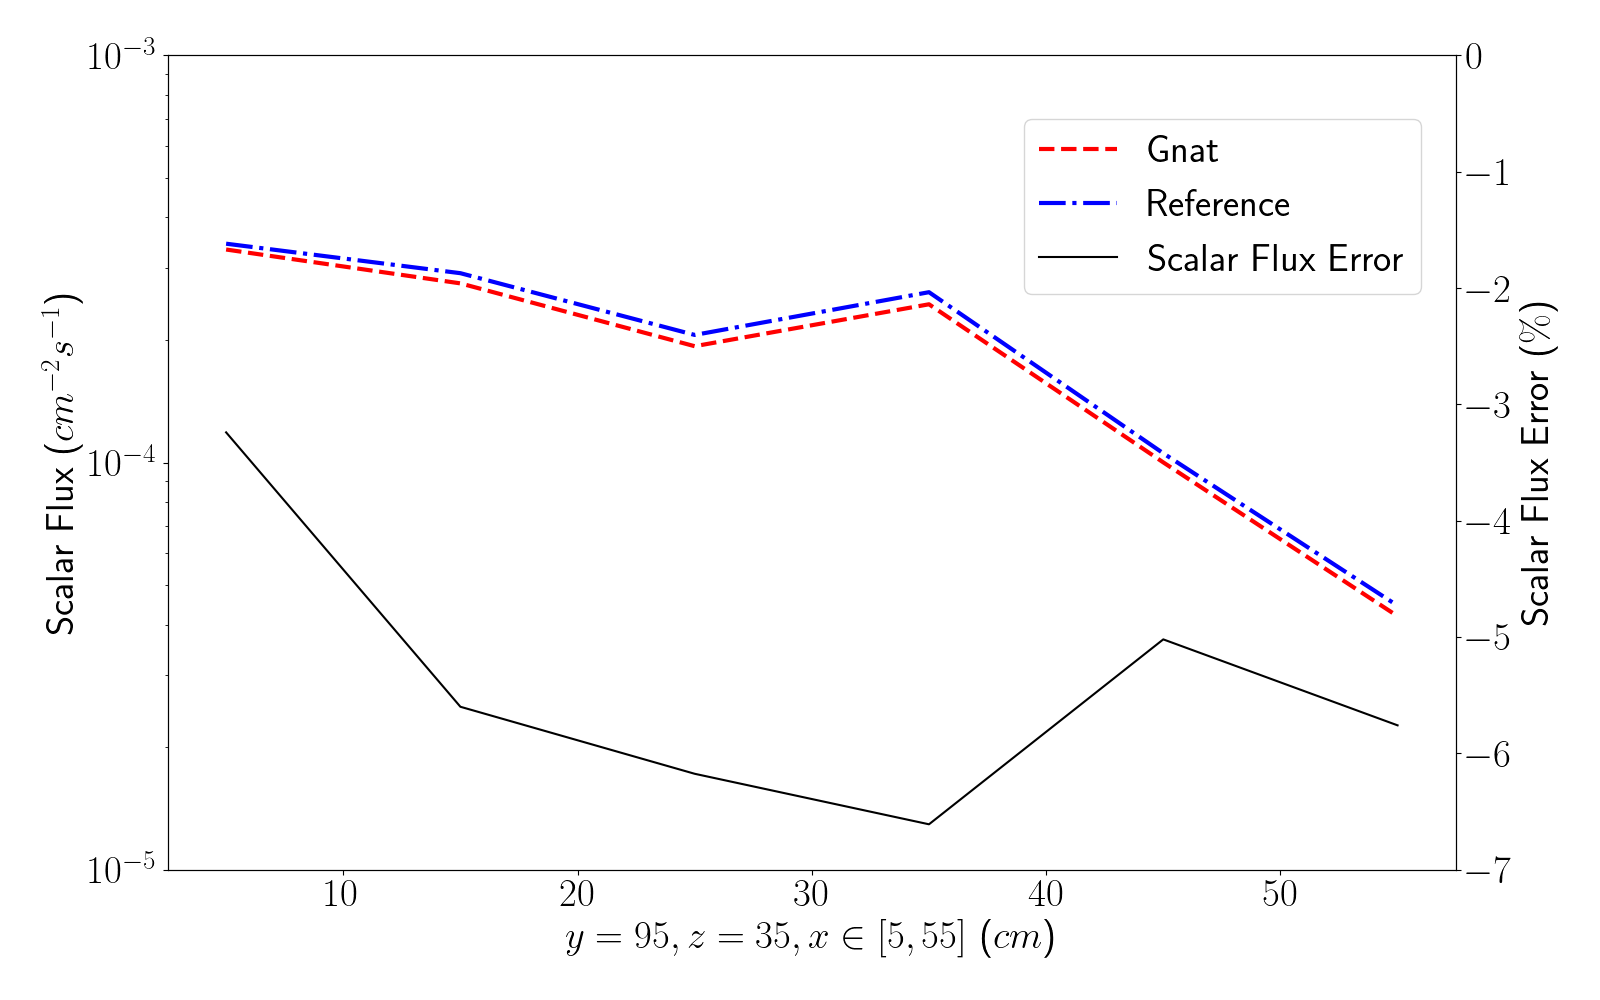
\includegraphics[width=\textwidth]{images/verification/sn_kobayashi/3/kobayashi_3c.png}
        \caption{Comparison with the benchmark problem. Reference taken from Kobayashi and Sugimura \cite{kobayashi_benchmarks}.}
        \label{fig:verification:sn_kobayashi_3c:line_plot}
    \end{subfigure}
    \caption{Results of the Kobayashi benchmark 3c.}
    \label{fig:verification:sn_kobayashi_3c}
\end{figure}

In general, the neutral particle transport solver matched the benchmark problems well. The relative error in the solutions can be explained by either a lack of a sufficiently refined spatial mesh or a need for additional angular directions to combat ray effects. The transport solver performed particularly well in optically thick diffusion regions such as the particle shield, which is expected as these regions are isotropic scattering dominant. The solver performed reasonably well when faced with jump discontinuities in cross section, however jump discontinuities which included particle sources resulted in additional error when compared with the reference solution of the first benchmark. Additional mesh refinement is considered necessary to better resolve material discontinuities in this radiation transport solver.

\subsection{The Ontario Tech Subcritical Assembly}
\label{verification:radiation_transport_sn:subcritical}

The third benchmark problem used to verify the accuracy of the \acrshort{sn} transport solver is two potential configurations of the Ontario Tech subcritical assembly \cite{ks_2024_subcritical}. These two problems were chosen for a verification study as they have to potential to be adapted to a validation benchmark in the future. The subcritical assembly is composed of $19\times 19$ square graphite elements. Each of these elements has a channel milled for either cylindrical fuel elements (natural uranium metal clad in aluminum), cylindrical graphite plugs, or cylindrical control rods (304 stainless steel). The central region of the assembly is the effective core while the remainder of the core is a reflector. The neutron sources used by the subcritical assembly consists of four americium-beryllium neutron sources with a combined intensity of $5\times 10^{7}\text{ s}^{\text{-1}}$ alongside a deuterium-tritium (D-T) neutron generator with an intensity of $1\times 10^{8}\text{ s}^{\text{-1}}$. The neutron sources are homogenized into a cube in the center of the subcritical assembly and the homogenized cross sections are assumed to be similar to that of air. The large size of the D-T neutron generator is likely to perturb the fluxes in the center of the assembly; a downside of this source homogenization is that the effects of these perturbations are not captured by this scheme. 
\begin{figure}[H]
    \centering
    \begin{subfigure}[b]{0.48\textwidth}
        \centering
        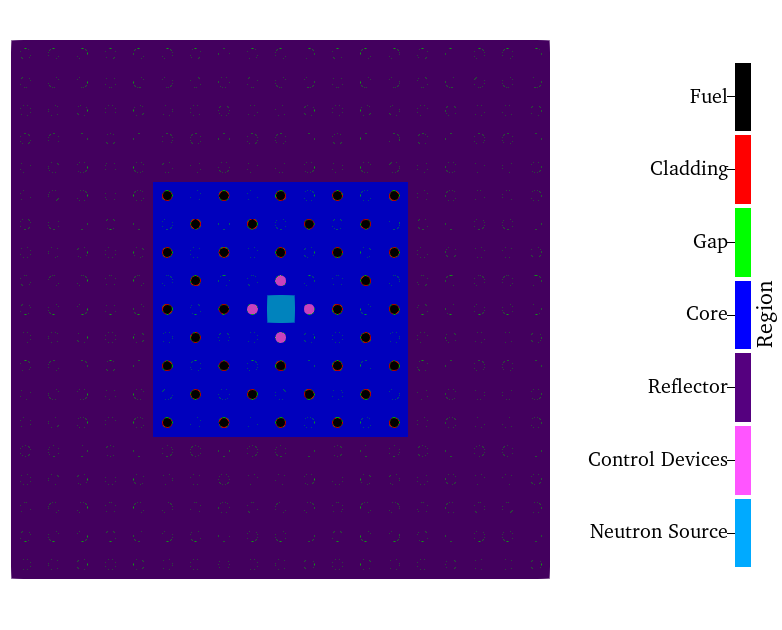
\includegraphics[width=\textwidth]{images/verification/subcritical/geo/subcritical_regions.png}
        \caption{2D lattice arrangement at $z = 0$.}
        \label{fig:subcritical_geo:2D_lattice}
    \end{subfigure}
    \hfill
    \begin{subfigure}[b]{0.48\textwidth}
        \centering
        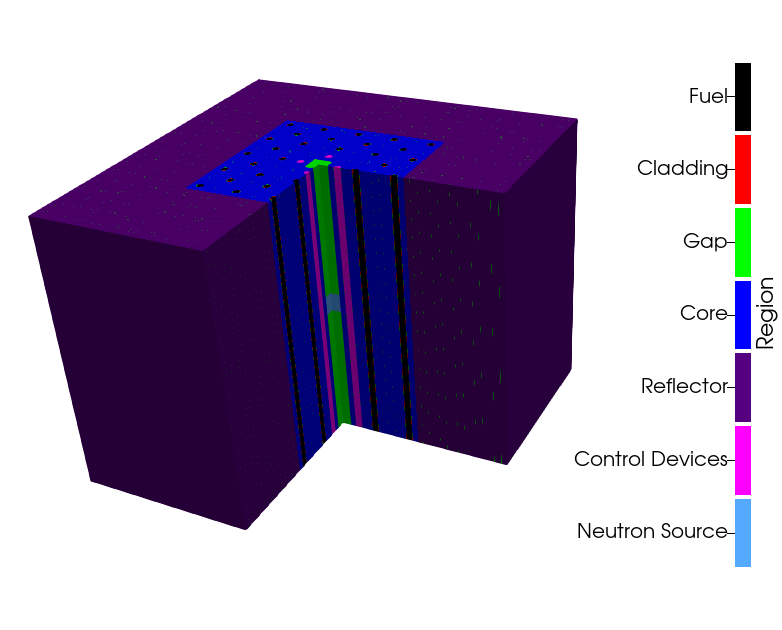
\includegraphics[width=\textwidth]{images/verification/subcritical/geo/3D_subcritical_regions.png}
        \caption{Full assembly sliced to reveal the neutron source.}
        \label{fig:subcritical_geo:full_geometry}
    \end{subfigure}
    \hfill
    \caption[The subcritical assembly benchmark geometry.]{The subcritical assembly benchmark geometry. Taken from Sawatzky and Atkinson \cite{ks_2024_subcritical}.}
    \label{fig:subcritical_geo}
\end{figure}

A lattice view of the subcritical assembly can be found in Figure~\ref{fig:subcritical_geo:2D_lattice} and a 3D view of the full core can be found in Figure~\ref{fig:subcritical_geo:full_geometry}. The first of the two subcritical assembly benchmark cases has the four control devices fully inserted. The second case has the control devices removed and replaced with graphite plugs. Both benchmark problems are criticality calculations where the eigenvalue $k_{eff}$ is the quantity of interest. The material properties of the assembly can be found in Table~\ref{table:subcritical_props} and the dimensions can be found in Figure~\ref{table:subcritical_dims}.
\begin{table}[H]
    \parbox{0.58\linewidth}
    {
        \centering
        \singlespacing
        \caption[Material properties of each region in the subcritical assembly.]{Material properties of each region in the subcritical assembly. Adapted from Sawatzky and Atkinson \cite{ks_2024_subcritical}.}
        \begin{tabular}{|c|c|c|}
            \hline
            \textbf{Region} & \makecell{\textbf{Density} \\ (g cm\textsuperscript{-3})} & \makecell{\textbf{Composition} \\(atom-fraction)}\\
            \hline
            \makecell{Fuel\\(Uranium Metal)} & $19.1$ & \makecell{\textsuperscript{235}U: $7.291\times 10^{-3}$\\\textsuperscript{238}U: $9.926\times 10^{-1}$}\\
            \hline
            \makecell{Cladding\\(Aluminum Metal)} & $2.699$ & \makecell{\textsuperscript{27}Al: $1.0$}\\
            \hline
            \makecell{Gap and \\Source\\(Air Filled)} & $1.2\times 10^{-3}$ & \makecell{\textsuperscript{14}N: $8.038\times 10^{-1}$\\\textsuperscript{15}N: $2.955\times 10^{-3}$\\\textsuperscript{16}O: $1.893\times 10^{-1}$}\\
            \hline
            \makecell{Core \& Reflector\\(Graphite)} & $1.91$ & \makecell{\textsuperscript{12}C: $9.889\times 10^{-1}$\\\textsuperscript{13}C: $1.111\times 10^{-2}$} \\
            \hline
            \makecell{Control Devices\\(304 Stainless Steel)} & $8.0$ & \makecell{\textsuperscript{12}C: $3.595\times 10^{-3}$\\\textsuperscript{28}Si: $1.792\times 10^{-2}$\\\textsuperscript{50}Cr: $9.121\times 10^{-3}$\\\textsuperscript{52}Cr: $1.759\times 10^{-1}$\\\textsuperscript{53}Cr: $1.995\times 10^{-2}$\\\textsuperscript{54}Cr: $4.965\times 10^{-3}$\\\textsuperscript{55}Mn: $1.987\times 10^{-2}$\\\textsuperscript{54}Fe: $3.761\times 10^{-2}$\\\textsuperscript{56}Fe: $5.905\times 10^{-1}$\\\textsuperscript{57}Fe: $1.363\times 10^{-2}$\\\textsuperscript{58}Fe: $1.815\times 10^{-3}$\\\textsuperscript{58}Ni: $6.963\times 10^{-2}$\\\textsuperscript{60}Ni: $2.682\times 10^{-2}$\\\textsuperscript{61}Ni: $1.166\times 10^{-3}$\\\textsuperscript{62}Ni: $3.718\times 10^{-3}$}\\
            \hline
        \end{tabular}
        \label{table:subcritical_props}
    }
    \hfill
    \parbox{0.40\linewidth}
    {
        \centering
        \singlespacing
        \caption[Dimensions of each region.]{Dimensions of each region. Adapted from Sawatzky and Atkinson \cite{ks_2024_subcritical}.}
        \begin{tabular}{|cc|}
            \hline
            \textbf{Dimension} & \textbf{Value}\\
            \hline
            Fuel Pin Diameter & $3.2766\text{ cm}$\\
            Cladding Thickness & $0.4064\text{ cm}$\\
            Block Length / Width & $10.16\text{ cm}$\\
            Channel Diameter & $3.96748\text{ cm}$\\
            Plug Diameter & $3.81\text{ cm}$\\
            Control Device Diameter & $3.81\text{ cm}$\\
            Assembly Height & $152.4\text{ cm}$\\
            \makecell{Homogenized Source \\ Length / Width / Height} & $10.16\text{ cm}$\\
            \makecell{Source Insertion Depth \\ (Top to Source Center)} & $71.12\text{ cm}$\\
            \hline
        \end{tabular}
        \label{table:subcritical_dims}
    }
\end{table}
\begin{table}[H]
    \singlespacing
    \centering
    \caption[Group structures used to generate multi-group cross sections for the subcritical assembly.]{Group structures used to generate multi-group cross sections for the subcritical assembly. Adapted from Agosta \cite{agosta_htgr}.}
    \begin{tabular}{|c|cccccccccccc|}
        \hline
          & \multicolumn{12}{c|}{}\\
         \makecell{\textbf{Upper Energy} \\ \textbf{Bound (eV)}} & \multicolumn{12}{c|}{\textbf{Group Structure}}\\
          & 26 & 21 & 18 & 15a & 15b & 15c & 15d & 15e & 12 & 9 & 6 & 3\\
         \hline
         $1.49\times 10^{7}$  & 1  & 1  & 1  & 1  & 1  & 1  & 1  & 1  & 1  & 1 & 1 & 1\\
         $7.41\times 10^{6}$  & 2  &    &    &    &    &    &    &    &    &   &   &  \\
         $3.68\times 10^{6}$  & 3  & 2  & 2  & 2  & 2  & 2  & 2  & 2  & 2  &   &   &  \\
         $6.72\times 10^{5}$  & 4  &    &    &    &    &    &    &    &    &   &   &  \\
         $1.11\times 10^{5}$  & 5  & 3  & 3  & 3  & 3  & 3  & 3  & 3  & 3  & 2 & 2 & 2\\
         $1.93\times 10^{4}$  & 6  & 4  & 4  & 4  & 4  &    &    &    & 4  &   &   &  \\
         $3.35\times 10^{3}$  & 7  &    &    &    &    &    &    &    &    &   &   &  \\
         $1.58\times 10^{3}$  & 8  & 5  & 5  &    &    & 4  &    &    &    &   &   &  \\
         $7.48\times 10^{2}$  & 9  & 6  & 6  & 5  & 5  &    & 4  & 4  & 5  & 3 &   &  \\
         $2.75\times 10^{2}$  & 10 & 7  & 7  & 6  & 6  & 5  &    &    & 6  & 4 &   &  \\
         $1.30\times 10^{2}$  & 11 & 8  & 8  & 7  & 7  &    & 5  & 5  & 7  & 5 & 3 &  \\
         $6.14\times 10^{1}$  & 12 & 9  &    &    & 8  & 6  &    &    &    &   &   &  \\
         $2.90\times 10^{1}$  & 13 & 10 & 9  & 8  & 9  &    & 6  &    &    &   &   &  \\
         $1.37\times 10^{1}$  & 14 & 11 & 10 & 9  &    &    &    &    & 8  & 6 &   &  \\
         $8.32\times 10^{0}$  & 15 & 12 & 11 & 10 & 10 & 7  & 7  & 7  & 9  &   &   &  \\
         $5.04\times 10^{0}$  & 16 &    &    &    &    &    &    &    &    &   &   &  \\
         $2.38\times 10^{0}$  & 17 & 13 & 12 & 11 & 11 & 8  & 8  & 8  & 10 & 7 & 4 & 3\\
         $1.29\times 10^{0}$  & 18 & 14 &    &    &    &    &    &    &    &   &   &  \\
         $6.50\times 10^{-1}$ & 19 & 15 & 13 & 12 & 12 & 9  & 9  & 9  & 11 & 8 & 5 &  \\
         $3.50\times 10^{-1}$ & 20 & 16 &    &    &    & 10 & 10 &    &    &   &   &  \\
         $2.00\times 10^{-1}$ & 21 & 17 & 14 & 13 & 13 & 11 & 11 & 10 &    &   &   &  \\
         $1.20\times 10^{-1}$ & 22 &    &    &    &    &    &    & 11 &    &   &   &  \\
         $8.00\times 10^{-2}$ & 23 & 18 & 15 & 14 & 14 & 12 & 12 & 12 &    &   &   &  \\
         $5.00\times 10^{-2}$ & 24 & 19 & 16 &    &    & 13 & 13 & 13 &    &   &   &  \\
         $2.00\times 10^{-2}$ & 25 & 20 & 17 & 15 & 15 & 14 & 14 & 14 & 12 & 9 & 6 &  \\
         $1.00\times 10^{-2}$ & 26 & 21 & 18 &    &    & 15 & 15 & 15 &    &   &   &  \\
         \hline
    \end{tabular}
    \label{table:subcritical_group_bnds}
\end{table}
The material properties and dimensions presented above were used to generate a model of the subcritical assembly in \texttt{OpenMC} \cite{openmc} for the purpose of generating multi-group cross sections for use with \acrshort{gnat} \cite{ks_2024_subcritical}. Agosta \cite{agosta_htgr} performed a literature view of multi-group cross section boundaries used for graphite moderated reactor systems, all of which will be used to generated cross sections for the subcritical assembly for the purposes of verifying \acrshort{gnat}. A summary of these group boundaries used can be found in Table~\ref{table:subcritical_group_bnds}. The \texttt{OpenMC} simulations used to generate the multi-group cross sections used 5,000 particles per generation, 10 generations per batch, 550 active batches and 50 inactive batches. This was sufficient to converge the fission source and reduce the standard deviations of the multi-group cross sections below 1\% \cite{ks_2024_subcritical}. These multi-group cross sections were then used with the multi-group mode of \texttt{OpenMC} to calculate the reference values of $k_{eff}$ that the \acrshort{sn} solver will be compared to, the results of which can be found in Sawatzky and Atkinson \cite{ks_2024_subcritical}.

The subcritical assembly benchmarks were meshed with 33,340 mixed tetrahedral and quadrilateral elements using the \acrshort{moose} \texttt{Reactor} module \cite{moose_reactor}. The mesh was split along three lines of symmetry: the x-y plane ($z = 0\text{cm}$), x-z plane ($y = 0\text{cm}$) and y-z plane ($x = 0\text{cm}$); this reduced the number of required elements and resulted in a 1/8\textsuperscript{th} core. Reflective boundary conditions are applied along these lines of symmetry to emulate the effect of the full assembly and vacuum boundary conditions are applied elsewhere. The resulting mesh is shown in Figure~\ref{table:subcritical_mesh}. 
\begin{figure}[H]
    \centering
    \begin{subfigure}[b]{0.48\textwidth}
        \centering
        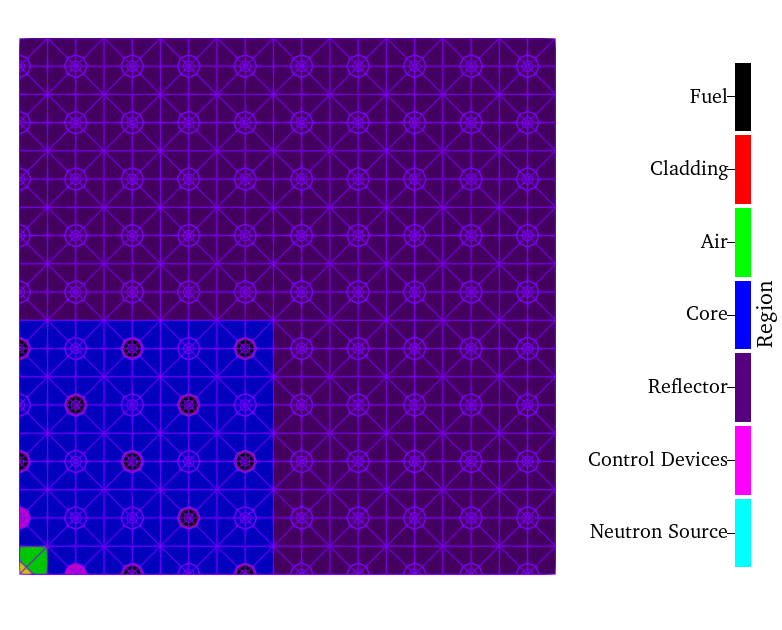
\includegraphics[width=\textwidth]{images/verification/subcritical/mesh/mesh_top.png}
        \caption{Top view of the generated mesh.}
        \label{table:subcritical_mesh_top}
    \end{subfigure}
    \hfill
    \begin{subfigure}[b]{0.48\textwidth}
        \centering
        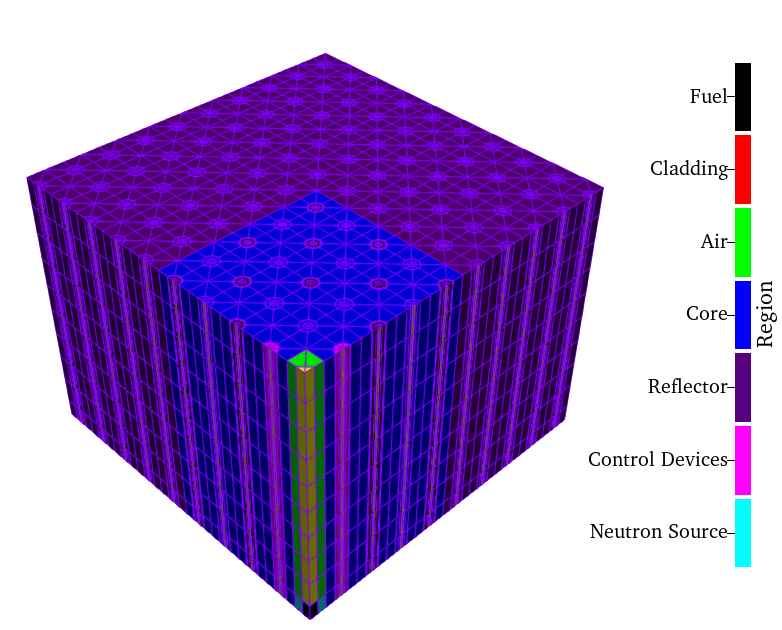
\includegraphics[width=\textwidth]{images/verification/subcritical/mesh/mesh_iso.png}
        \caption{Full view of the 1/8\textsuperscript{th} core.}
        \label{table:subcritical_mesh_iso}
    \end{subfigure}
    \hfill
    \caption[Meshed subcritical assembly geometry.]{Meshed subcritical assembly geometry. Taken from Sawatzky and Atkinson \cite{ks_2024_subcritical}.}
    \label{table:subcritical_mesh}
\end{figure}
\noindent Linear Lagrange finite element basis functions were used. All benchmark cases used the \acrshort{moose} \texttt{Eigenvalue} solver with the \acrshort{pjfnk} method using 600 \acrshort{gmres} vectors, preconditioning was provided by the hypre package BoomerAMG. Each simulation used a Gauss-Chebyshev quadrature with three polar angles and three azimuthal angles; this was considered appropriate as graphite moderated systems tend to be diffuse over the majority of the energy spectrum and do not exhibit strong streaming effects \cite{ks_2024_subcritical}. In addition to the angular resolution of the problem, the scattering anisotropy must also be considered. Transport corrected isotropic scattering cross sections were found to be as accurate as linear anisotropic scattering cross sections for this assembly, and increases in the degree of anisotropy was not found to significantly improve the accuracy of $k_{eff}$ calculations \cite{ks_2024_subcritical}. Evaluating the scattering kernel requires less computing time when isotropic scattering is assumed, and so transport corrected scattering cross sections are selected for this problem. Finally, an initial residual vector magnitude of $1.000105$ was reported by \acrshort{petsc}. This led to the use of a relative convergence criteria of $10^{-8}$ to ensure that the magnitude of the final residual vector was below $10^{-8}$ on convergence. Testing with the three group problem indicated that additional tightening of the relative convergence criteria was not required. The results of these criticality calculations alongside the absolute difference with the multi-group Monte Carlo results obtained by Sawatzky and Atkinson \cite{ks_2024_subcritical} can be found in Table~\ref{table:k_eff_gnat_vs_mc}, where $\Delta k_{eff} =  (k_{eff, \text{OpenMC}} - k_{eff, \text{Gnat}})\times 10^{-5}$ (pcm).
\begin{table}[H]
    \singlespacing
    \centering
    \caption{$k_{eff}$ predicted by \acrshort{gnat} vs multi-group \texttt{OpenMC} for both the rodded and unrodded assembly.}
    \begin{tabular}{|c|cccc|}
        \hline
        & \multicolumn{2}{c}{\textbf{Rodded Case}} & \multicolumn{2}{c|}{\textbf{Unrodded Case}}\\
        \textbf{G} & Gnat $k_{eff}$ & \makecell{$\Delta k_{eff}$ \\ (pcm)} & Gnat $k_{eff}$ & \makecell{$\Delta k_{eff}$ \\ (pcm)}\\
        \hline
        3   & $0.671352$ & $-214.5$ & $0.724530$ & $144.3$\\
        6   & $0.665454$ & $-170.5$ & $0.719861$ & $189.3$\\
        9   & $0.663403$ & $-161.8$ & $0.718573$ & $245.0$\\
        12  & $0.660716$ & $-148.0$ & $0.716210$ & $273.9$\\
        15a & $0.659284$ & $-147.1$ & $0.714858$ & $247.1$\\
        15b & $0.659357$ & $-185.0$ & $0.714962$ & $240.2$\\
        15c & $0.659720$ & $-203.4$ & $0.714931$ & $250.9$\\
        15d & $0.659908$ & $-185.0$ & $0.715010$ & $220.2$\\
        15e & $0.660165$ & $-179.9$ & $0.715167$ & $226.0$\\
        18  & $0.658896$ & $-176.3$ & $0.714572$ & $273.2$\\
        21  & $0.658691$ & $-157.5$ & $0.714353$ & $260.4$\\
        26  & $0.654831$ & $-123.9$ & $0.710522$ & $262.5$\\
        \hline
    \end{tabular}
    \label{table:k_eff_gnat_vs_mc}
\end{table}
Table~\ref{table:k_eff_gnat_vs_mc} shows that the deterministic model solved by the \acrshort{sn} transport solver over predicts $k_{eff}$ in the rodded case and under predicts $k_{eff}$ in the unrodded case when compared to the multi-group Monte Carlo reference solution. This behavior is consistent regardless of the number of energy groups or group boundaries, indicating that this is a systematic issue with the benchmark problem as implemented. A possible cause for this discrepancy is the coarse mesh used in the deterministic simulation, alongside the low order angular quadrature set. As the \acrshort{saaf} equations are not locally conservative, a poorly resolved mesh near spatially heterogeneous regions such as the fuel and control devices will result in large changes to $k_{eff}$. Ray effects appear in the fast neutron fluxes in the numerical solution \cite{ks_2024_subcritical}, which increases $|\Delta k_{eff}|$. These ray effects are caused by the lower total cross sections in the fast neutron energy groups. Future works should include testing with a more resolved mesh and a higher order angular quadrature set to ensure that the \acrshort{sn} solver converges to the multi-group Monte Carlo results. 

\section{Ray Traced Uncollided Flux}
\label{verification:radiation_transport_rt}

This section details the verification strategy used for the ray traced uncollided flux method implemented in \acrshort{gnat}. Verification begins by determining the accuracy and rate of convergence of the method using a simple analytical transport problem. This is then followed by the third Kobayashi benchmark, which is used to determine the effectiveness of the ray effect mitigation strategy when coupled with the \acrshort{sn} transport solver.

\subsection{3D Analytical Transport Problem}
\label{verification:radiation_transport_rt:3D_anal}

Consider a 3D infinite absorbing medium with a point particle source placed at the origin ($\vec{r}_{s} = \{0,0,0\}$). The radiation transport equation for this can can be written as the following:
\begin{equation}\label{eq:3D_inf_transport}
    \hat{\Omega}\cdot\vec{\nabla}\psi(\vec{r}, \hat{\Omega}) + \Sigma_{t}\psi(\vec{r},\hat{\Omega}) = \frac{q}{4\pi}\delta(\vec{r}),\,\,\,\,x\in[-\infty, \infty],y\in[-\infty, \infty],z\in[-\infty, \infty]\text{.}
\end{equation}
The solution to this transport problem can be obtained using Green's functions, and takes the following form:
\begin{equation}
    \Phi_{a}(\vec{r}) = \frac{q e^{-\Sigma_{t}||\vec{r}||}}{4\pi ||\vec{r}||}
\end{equation}
\cite{computational_methods}. This work sets $\Sigma_{t}$ to either $0.0$ cm\textsuperscript{-1} or $0.01$ cm\textsuperscript{-1} to determine the effect of cross section on the convergence of the ray traced scalar fluxes. The size of the domain is set to either 2 cm x 2 cm x 2 cm or 2000 cm x 2000 cm x 2000 cm to determine the impact of the problem length scale on the accuracy of the solution. The mesh on which the ray tracing solution is projected on contains 8,000 elements, where each element has a sided length of 0.1 cm for the 2 cm domain and 100 cm for the 2000 cm domain. The ray tracing mesh takes the projection mesh and uniformly refines it once. Both of these meshes are uniformly refined twice to determine the impact of mesh density on the accuracy of the solution. No spatial quadrature is used when computing the average fluxes; rays are traced to the element centroid and the resulting point-wise scalar flux is then divided by the element volume. The results of this case can be found in Figure~\ref{fig:verification:rt:void} and Figure~\ref{fig:verification:rt:shield} below, where the $L_{2}$ error metric is defined as:
\begin{equation}\label{eq:l2_error_rt}
    e_{L2} = \sqrt{\int_{V}\Big(\Phi(\vec{r})- \Phi_{a}(\vec{r})\Big)^{2}\,dV}\text{,}
\end{equation}
and $h$ is the average vertex separation in all elements. 

The convergence plots below exclude a region near the point source due to the singularity in the analytical solution as $||\vec{r}||$ approaches zero. To ensure that this exclusion has no impact on the measured rate of convergence the size of the near source region was set to either 10\% of the domain, 20\% of the domain, or 50\% of the domain. It can be seen that the overall $L_{2}$ error is several orders of magnitude lower in the 2000 cm domain when compared to the 2 cm domain. This is likely due to the coarse mesh resolution of the 2000 cm domain as few elements are placed near the source. Variations in the scalar flux within this region are more rapid and are therefore more susceptible to error with the average flux approach. The exclusion of even a 10\% near source region during the calculation of the $L_{2}$ compounds this issue. The rate of convergence of this technique was obtained by performing a a linear regression on the logarithm of the $L_{2}$ error and the logarithm of the mesh-average minimum vertex separation ($h$) at each mesh refinement step. The rates of convergence can be found in the legends of Figure~\ref{fig:verification:rt:void} and Figure~\ref{fig:verification:rt:shield}; it an be seen that the rate of convergence is first-order. Harbour \cite{harbour_uncollided} determined that this is the anticipated order of convergence for this approach, and so this finding lends credibility to the implementation being correct. This rate of convergence is unaffected by the cross section of the domain, size of the domain, and the size of the near source region. The exception to this is the 2000 cm absorber, where the rate of convergence is $1.2$. This is likely due to the slow variation in the solution caused by the near-full attenuation of the point source this far removed from the origin.

% 0.495
\begin{figure}[H]
    \centering
    \begin{subfigure}[b]{\textwidth}
        \centering
        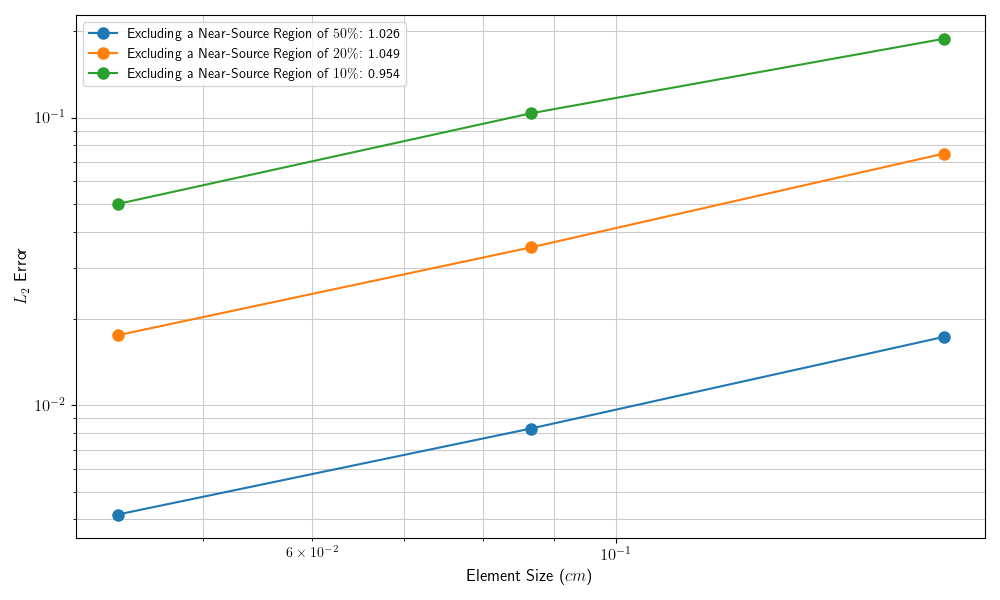
\includegraphics[width=\textwidth]{images/verification/rt_anal/vacuum_point_source_convergence_2.png}
        \caption{$L_{2}$ error for the ray traced uncollided flux technique for a 2 cm void.}
        \label{fig:verification:rt:void:2}
    \end{subfigure}
    \hfill
    \begin{subfigure}[b]{\textwidth}
        \centering
        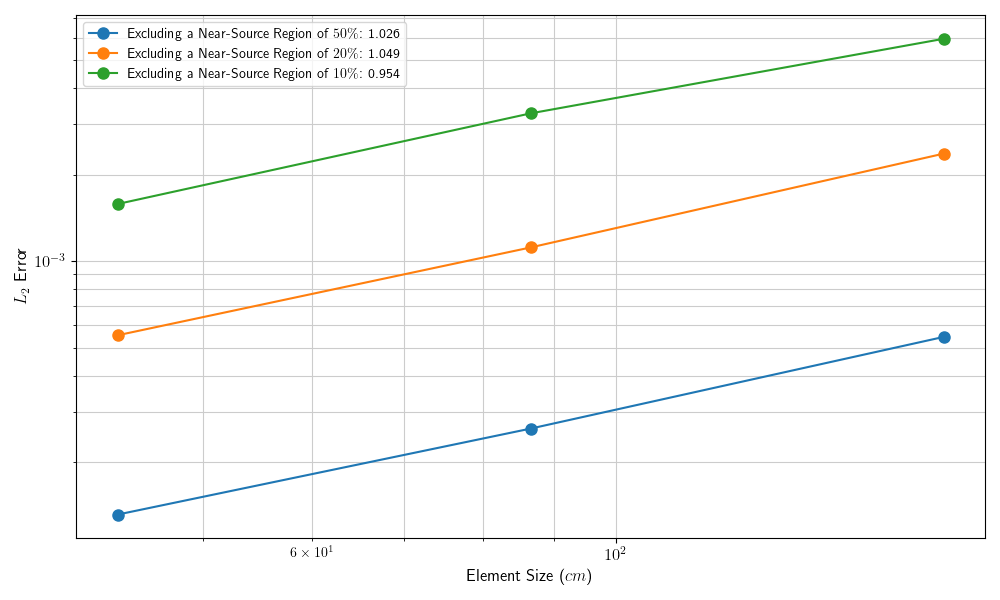
\includegraphics[width=\textwidth]{images/verification/rt_anal/vacuum_point_source_convergence_2000.png}
        \caption{$L_{2}$ error for the ray traced uncollided flux technique for a 2000 cm void.}
        \label{fig:verification:rt:void:2000}
    \end{subfigure}
    \caption{Convergence of the ray traced technique in a void.}
    \label{fig:verification:rt:void}
\end{figure}

\begin{figure}[H]
    \centering
    \begin{subfigure}[b]{\textwidth}
        \centering
        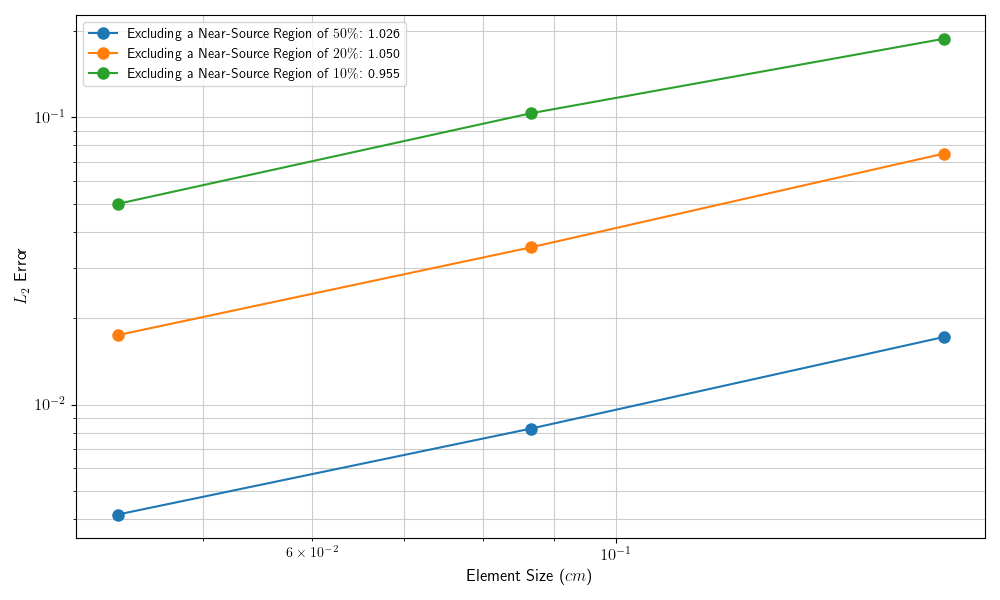
\includegraphics[width=\textwidth]{images/verification/rt_anal/shield_point_source_convergence_2.png}
        \caption{$L_{2}$ error for the ray traced uncollided flux technique for a 2 cm absorber.}
        \label{fig:verification:rt:shield:2}
    \end{subfigure}
    \hfill
    \begin{subfigure}[b]{\textwidth}
        \centering
        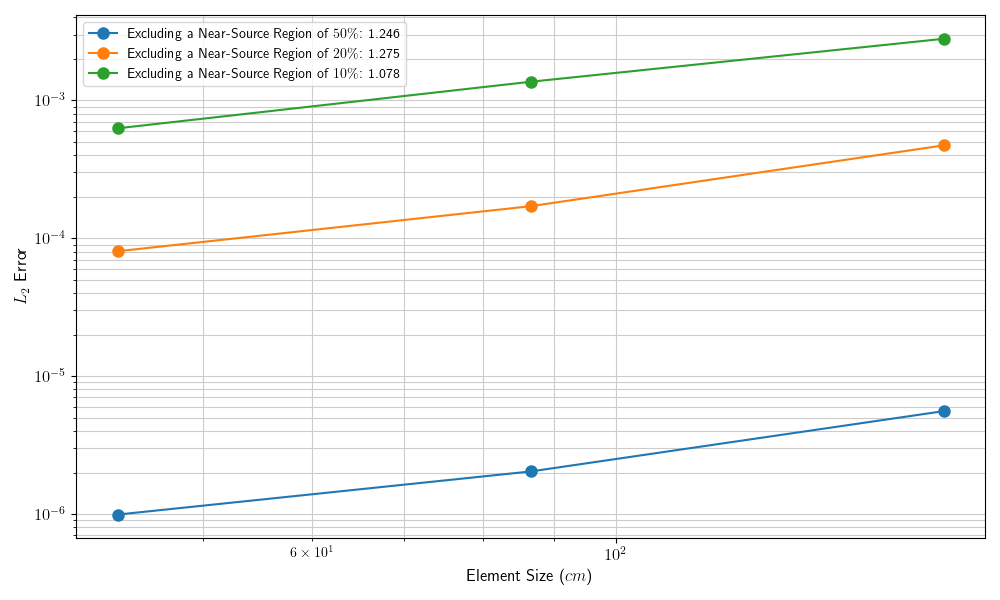
\includegraphics[width=\textwidth]{images/verification/rt_anal/shield_point_source_convergence_2000.png}
        \caption{$L_{2}$ error for the ray traced uncollided flux technique for a 2000 cm absorber.}
        \label{fig:verification:rt:shield:2000}
    \end{subfigure}
    \caption{Convergence of the ray traced technique in a light absorber.}
    \label{fig:verification:rt:shield}
\end{figure}

\subsection{The Third Kobayashi Benchmark with Ray Tracing}
\label{verification:radiation_transport_rt:kobayashi}

This verification case repeats the third Kobayashi benchmark where the ray traced uncollided flux method is used to remove ray effects. The problem is initially solved with a Gauss-Chebyshev quadrature set using 5 polar angles and 5 azimuthal angles per octant of the unit sphere, resulting in a total of 200 angular directions. The remaining parameters of the solution are the same as Section~\ref{verification:radiation_transport_rt:kobayashi}. The method of ray tracing was then used to solve for the uncollided flux, which was passed as the first collision source into the \acrshort{sn} solver to resolve the collided flux with the same angular quadrature set. The ray tracing mesh was once refined from the mesh used in Section~\ref{verification:radiation_transport_rt:kobayashi}, resulting in a total of 184,320 elements. Out of these elements, 512 contained the volumetric source. This resulted in the need to trace 94,371,328 rays from the volume sources to the non-source elements using the cell-centered approach. A Gauss-Chebyshev quadrature with 30 polar angles and 30 azimuthal angles per octant of the unit sphere was used to compute the contribution of a source element to itself. In total, this mitigation strategy required 98,057,728 rays to compute the uncollided flux. The results of this ray effect mitigation approach can be found in Figures~\ref{fig:verification:rt:kobayashi_3a} to \ref{fig:verification:rt:kobayashi_3c}.

Viewing the results below, it can be seen that this lower-order ray traced uncollided flux method is reasonably effective at removing ray effects from the third Kobayashi benchmark. Figure~\ref{fig:verification:rt:kobayashi_3a} shows how the error in the solution increases over the length of the duct up to a maximum of 10\%. The error then rapidly increases in the shielded region to -30\%. Ray effect mitigation replaces this error with a relatively constant error over the length of the duct which peaks right after the particle source and near the transition between duct and shield. This behavior is likely due to rapid variations of the scalar flux which are not well represented by the average fluxes in this numerical result. Figure~\ref{fig:verification:rt:kobayashi_3b} shows how the rapid variations in the scalar flux near the particle shield canont be accurately captured by the first order accurate uncollided flux approach, resulting in an accuracy penalty when compared to the \acrshort{sn} results. The benefits of ray effect mitigation become more apparent in Figure~\ref{fig:verification:rt:kobayashi_3c} when plotting over the duct after it undergoes several right angle turns. The ray effect mitigation approach decreases the error from a maximum of 40\% to 24\%. The distribution of the scalar flux in Figure~\ref{fig:verification:rt:kobayashi_3c:rt} more closely represents the reference solution then the scalar flux in Figure~\ref{fig:verification:rt:kobayashi_3c:no_rt}. This indicates that this low order ray effect mitigation approach is the most effective for deep penetration problems when many \acrshort{sn} directions cannot be used. In general, the ray traced solution matches the reference solution well when considering the lack of a spatial quadrature when computing the average uncollided scalar flux and the use of a coarse mesh.

\begin{figure}[H]
    \centering
    \begin{subfigure}[b]{\textwidth}
        \centering
        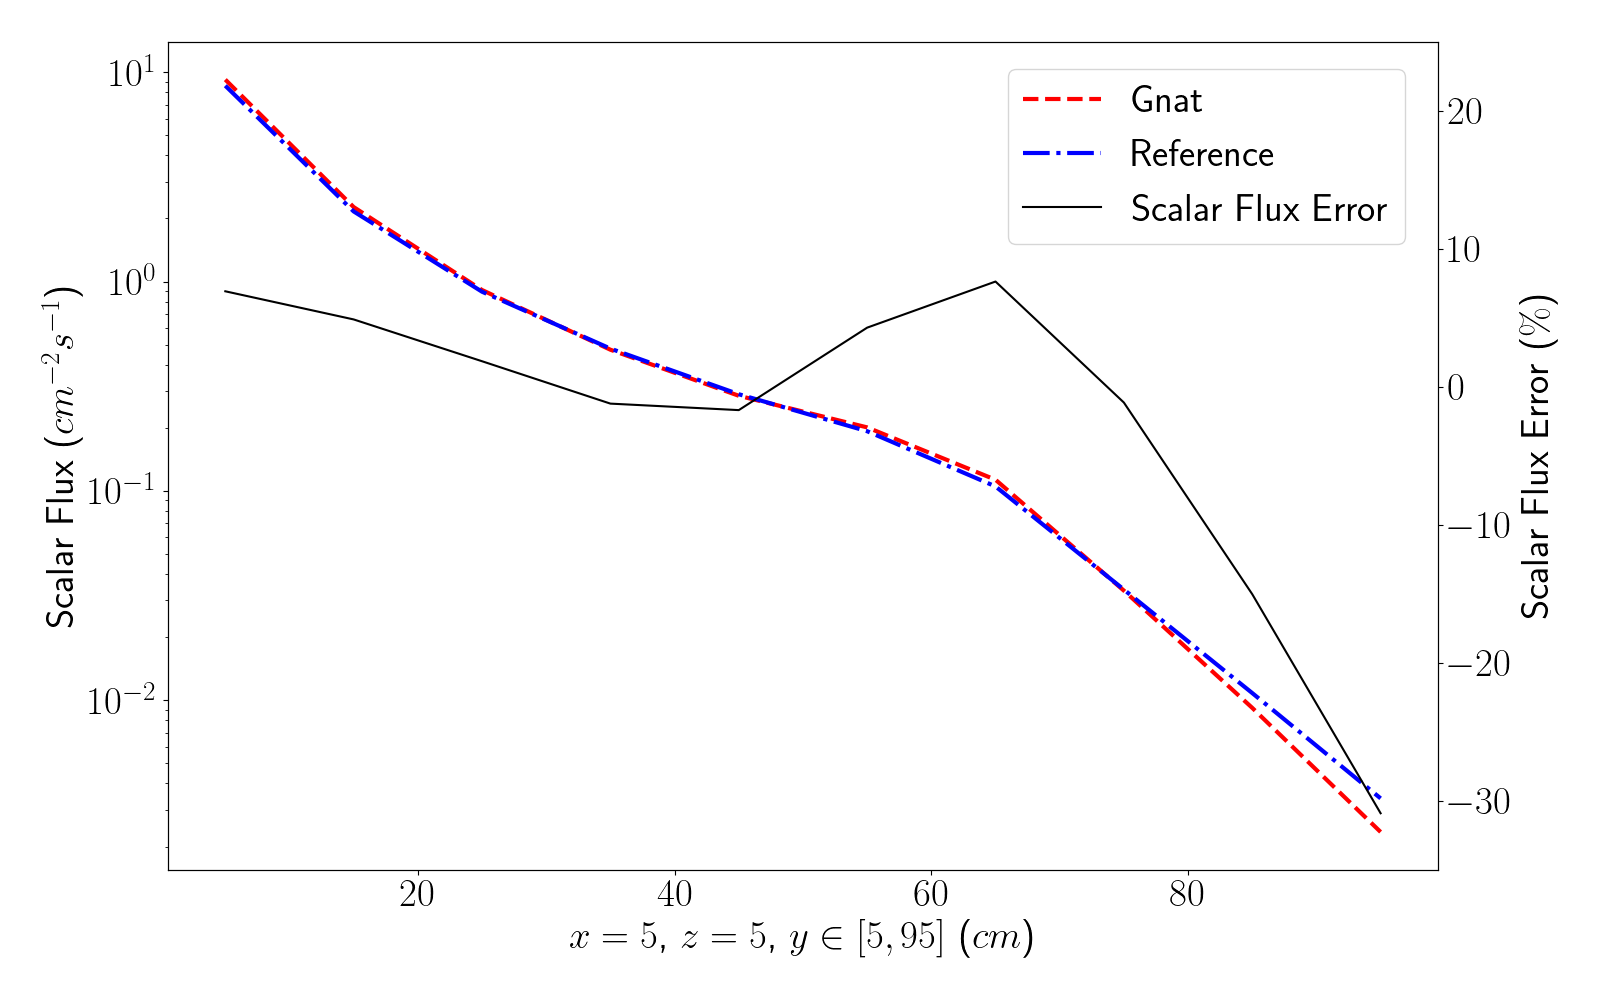
\includegraphics[width=0.8\textwidth]{images/verification/rt_kobayashi/kobayashi_3a_no_rt.png}
        \caption{No ray effect mitigation. Reference taken from Kobayashi and Sugimura \cite{kobayashi_benchmarks}.}
        \label{fig:verification:rt:kobayashi_3a:no_rt}
    \end{subfigure}
    \hfill
    \begin{subfigure}[b]{\textwidth}
        \centering
        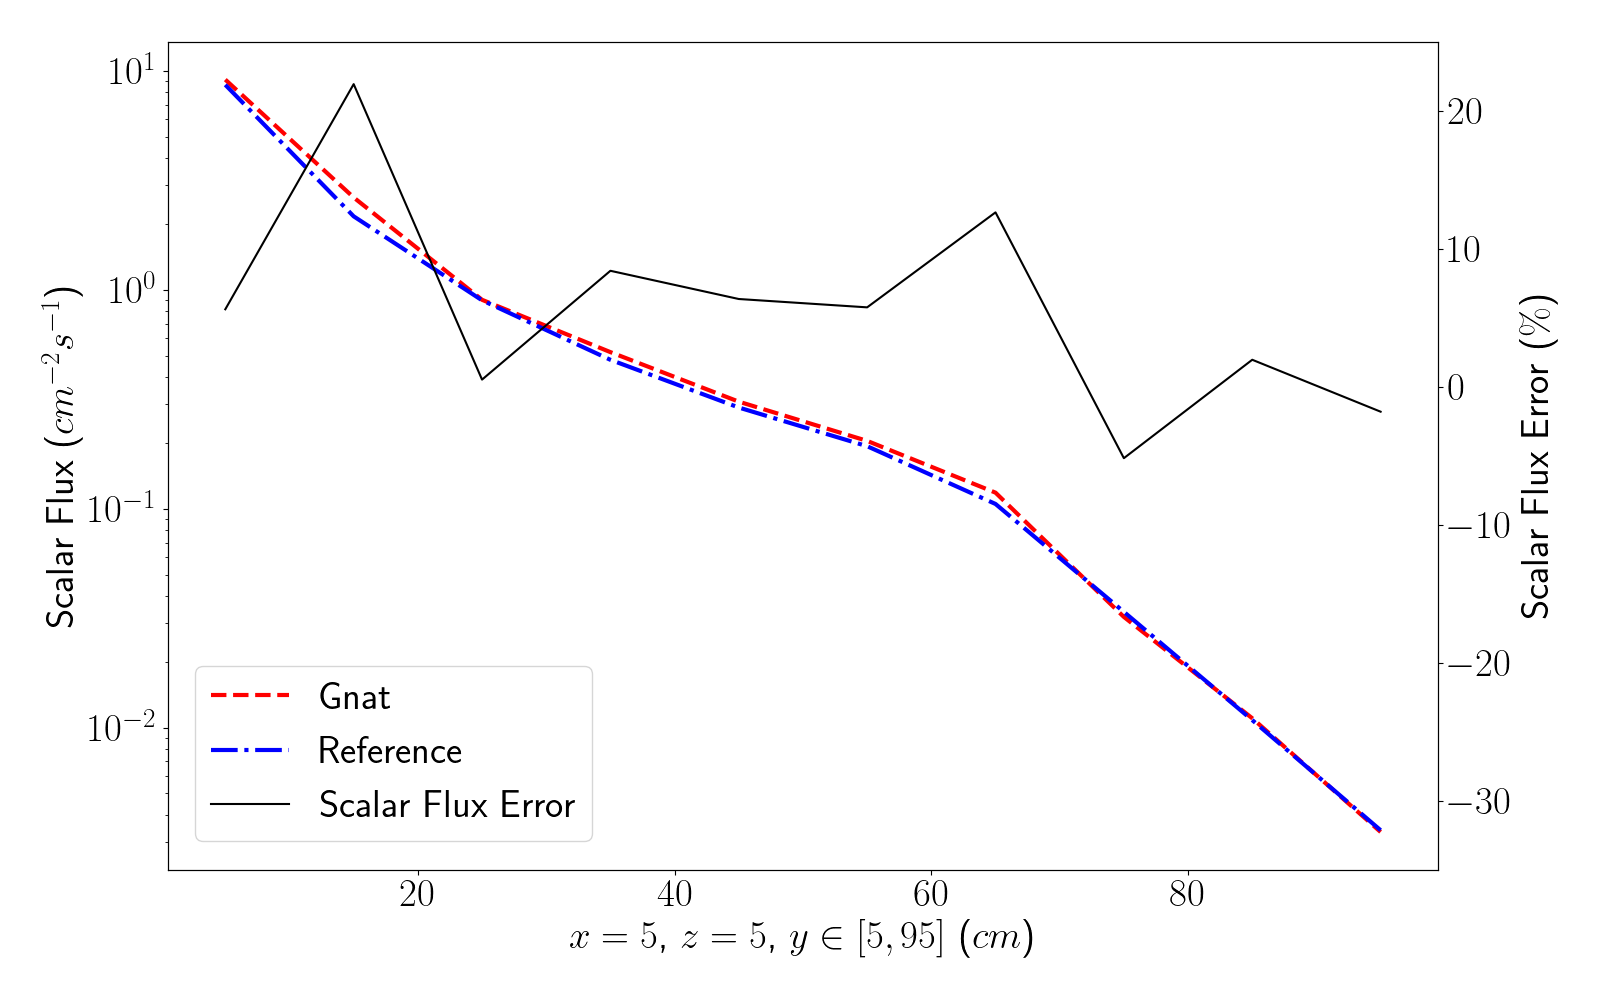
\includegraphics[width=0.8\textwidth]{images/verification/rt_kobayashi/kobayashi_3a_rt.png}
        \caption{With ray effect mitigation. Reference taken from Kobayashi and Sugimura \cite{kobayashi_benchmarks}.}
        \label{fig:verification:rt:kobayashi_3a:rt}
    \end{subfigure}
    \caption{Ray effect mitigation applied to the third Kobayashi benchmark, case a.}
    \label{fig:verification:rt:kobayashi_3a}
\end{figure}

\begin{figure}[H]
    \centering
    \begin{subfigure}[b]{\textwidth}
        \centering
        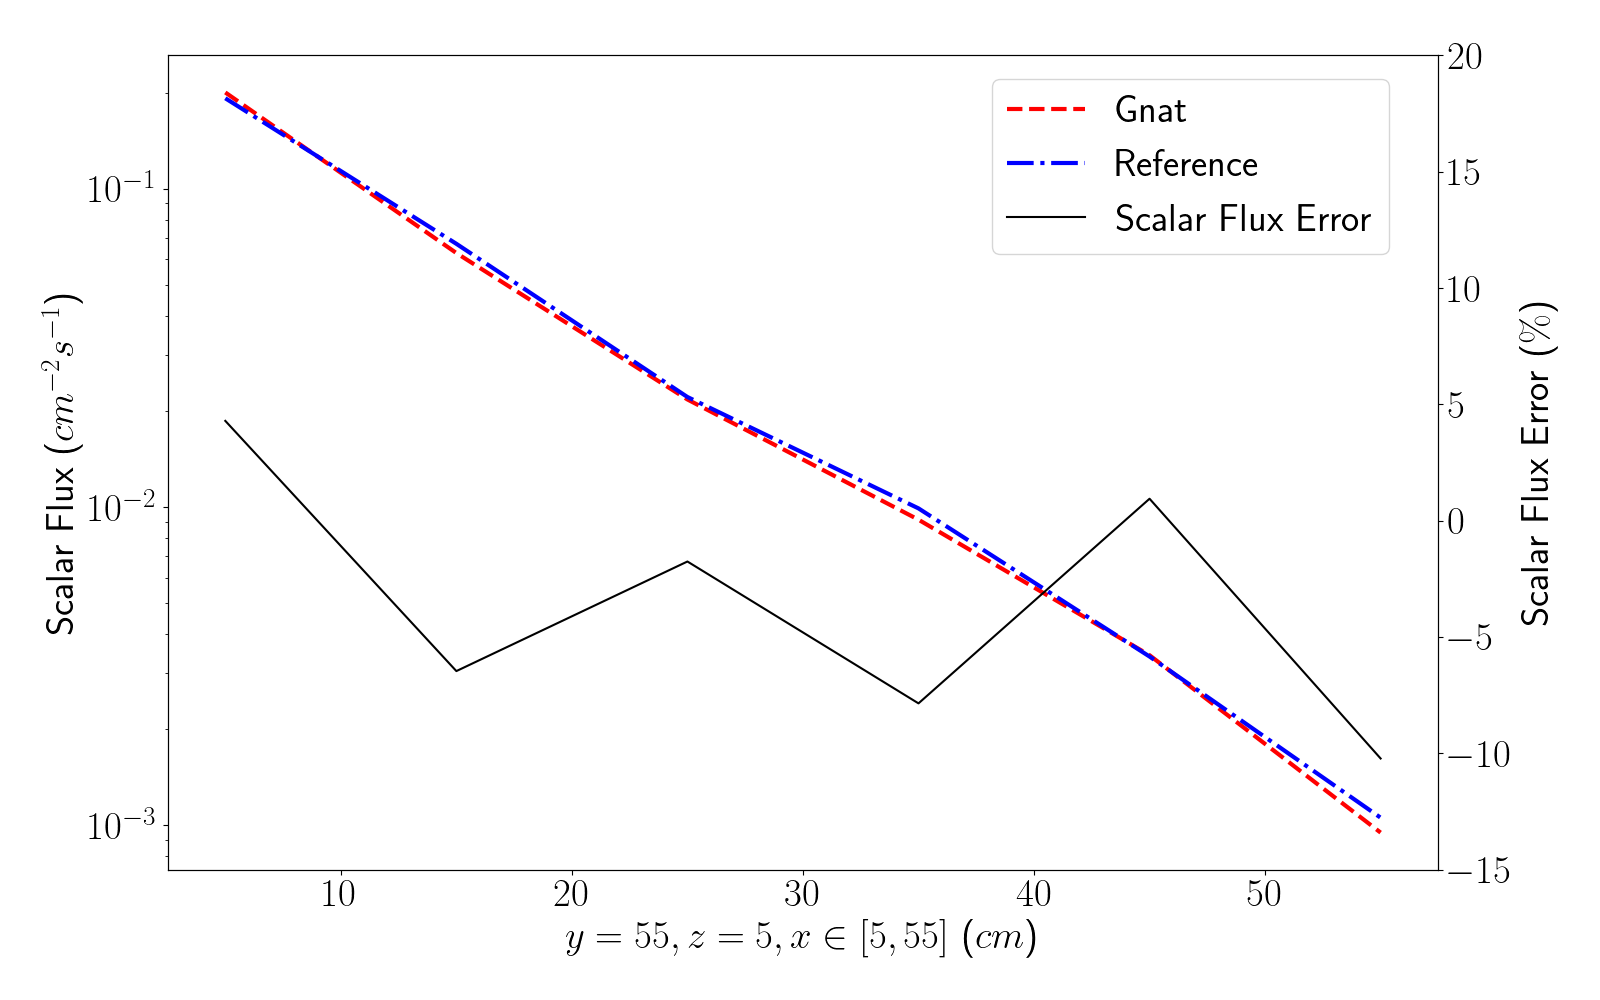
\includegraphics[width=0.8\textwidth]{images/verification/rt_kobayashi/kobayashi_3b_no_rt.png}
        \caption{No ray effect mitigation. Reference taken from Kobayashi and Sugimura \cite{kobayashi_benchmarks}.}
        \label{fig:verification:rt:kobayashi_3b:no_rt}
    \end{subfigure}
    \hfill
    \begin{subfigure}[b]{\textwidth}
        \centering
        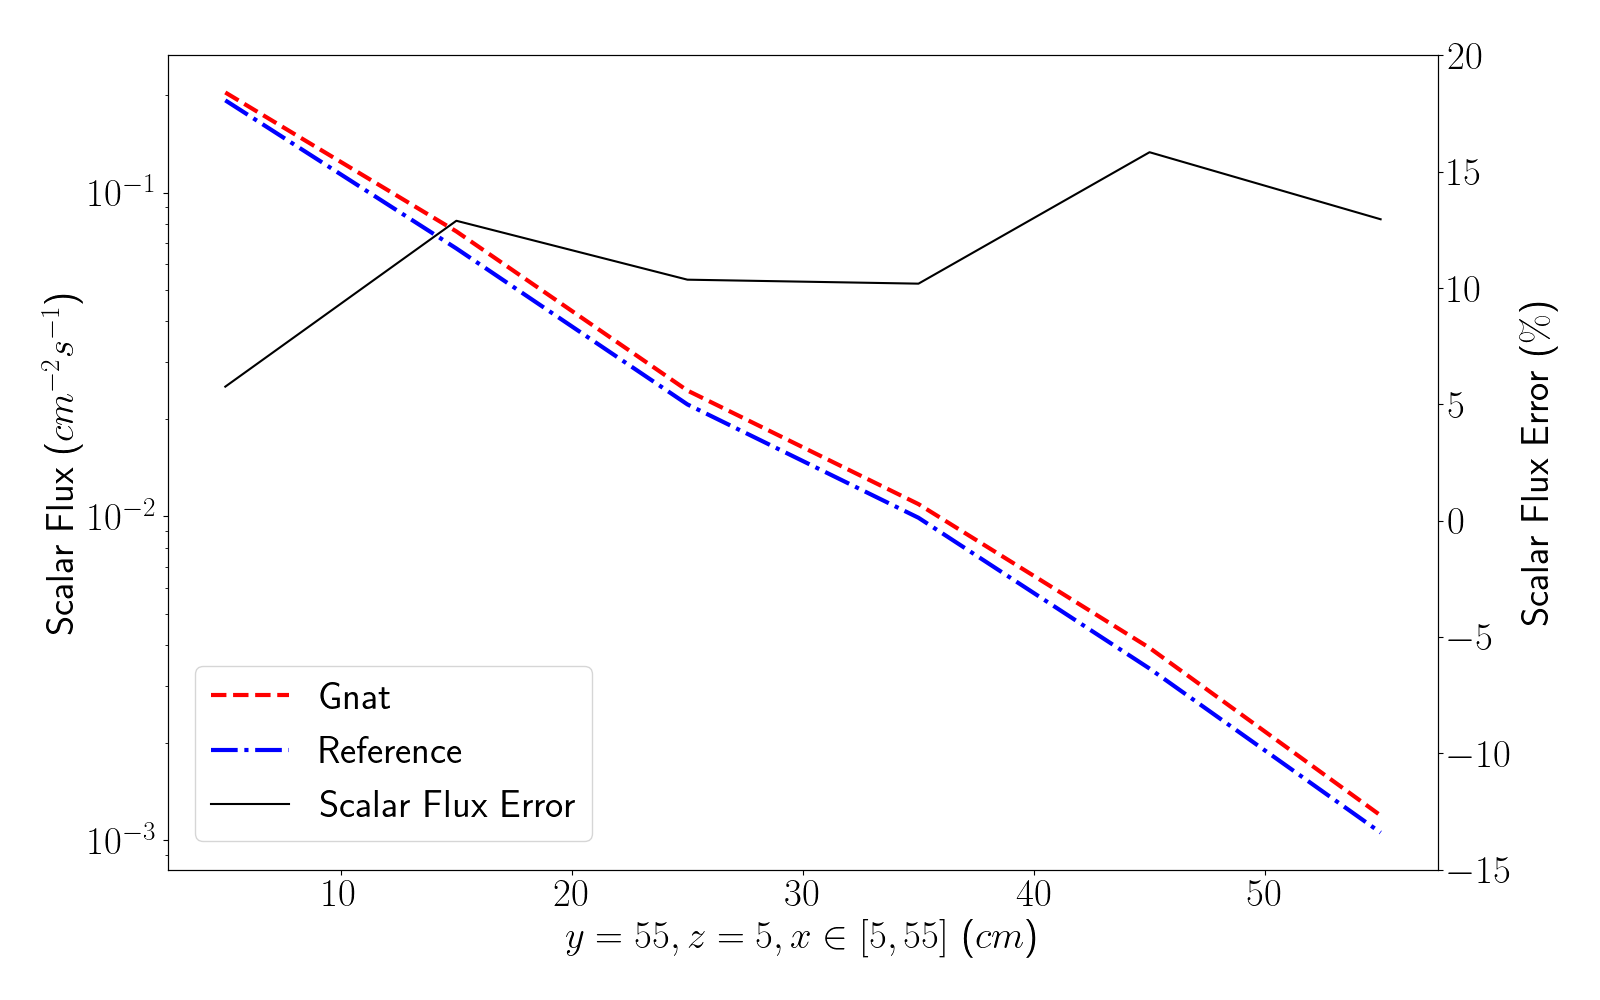
\includegraphics[width=0.8\textwidth]{images/verification/rt_kobayashi/kobayashi_3b_rt.png}
        \caption{With ray effect mitigation. Reference taken from Kobayashi and Sugimura \cite{kobayashi_benchmarks}.}
        \label{fig:verification:rt:kobayashi_3b:rt}
    \end{subfigure}
    \caption{Ray effect mitigation applied to the third Kobayashi benchmark, case b.}
    \label{fig:verification:rt:kobayashi_3b}
\end{figure}

\begin{figure}[H]
    \centering
    \begin{subfigure}[b]{\textwidth}
        \centering
        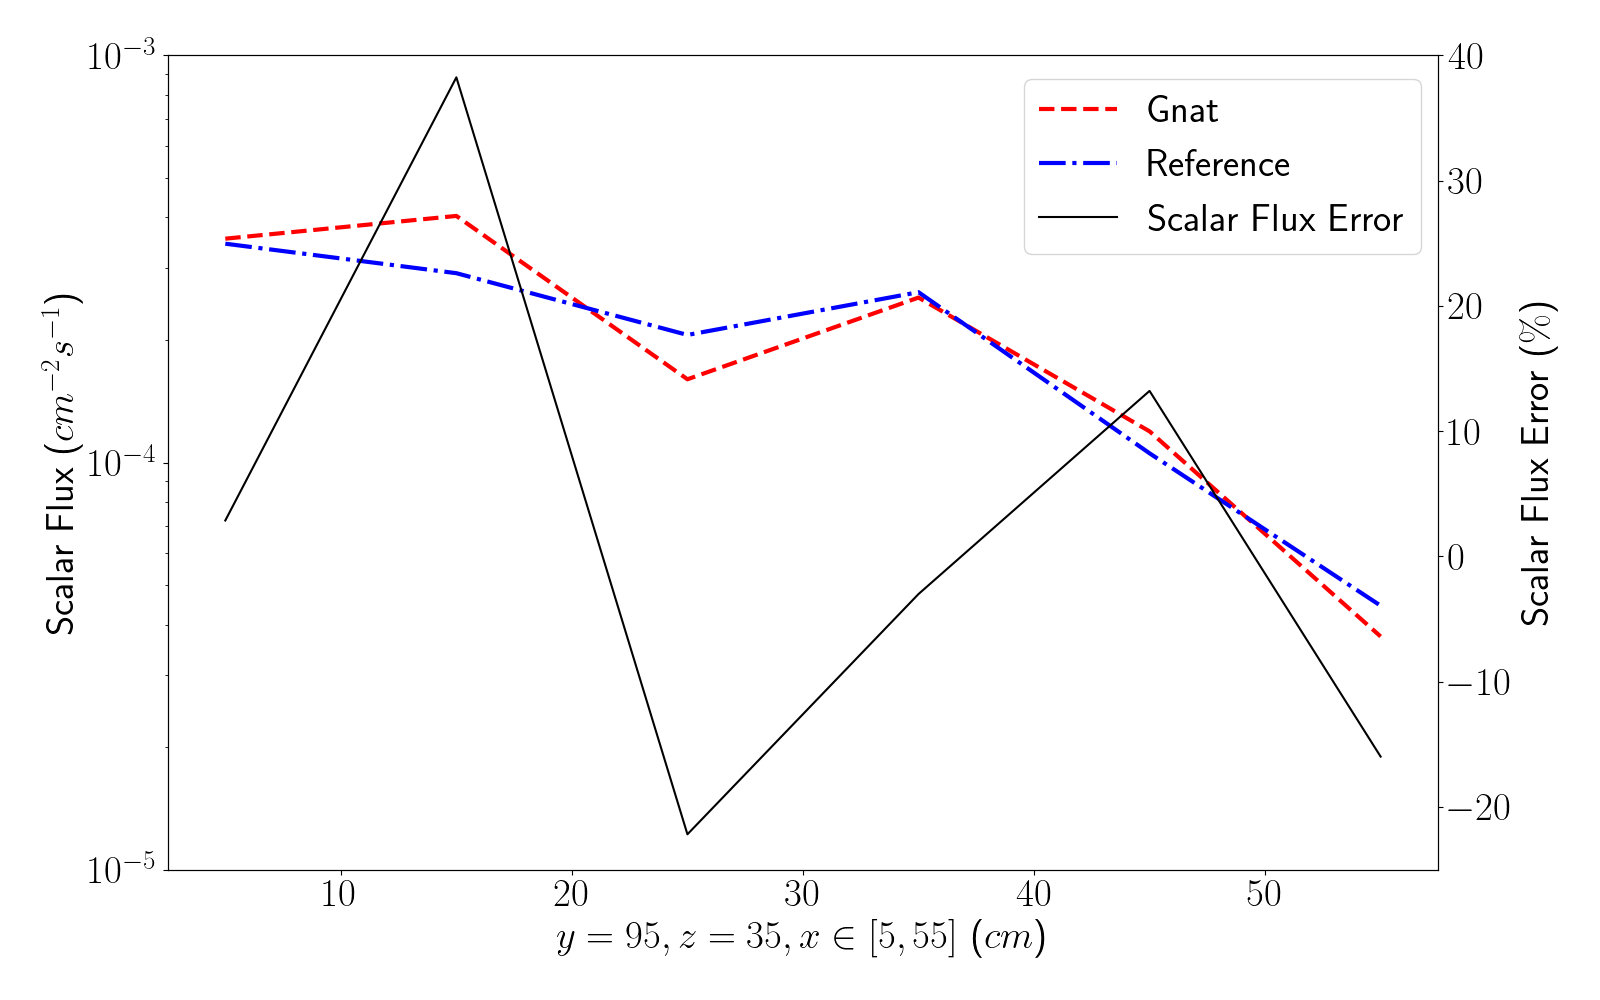
\includegraphics[width=0.8\textwidth]{images/verification/rt_kobayashi/kobayashi_3c_no_rt.png}
        \caption{No ray effect mitigation. Reference taken from Kobayashi and Sugimura \cite{kobayashi_benchmarks}.}
        \label{fig:verification:rt:kobayashi_3c:no_rt}
    \end{subfigure}
    \hfill
    \begin{subfigure}[b]{\textwidth}
        \centering
        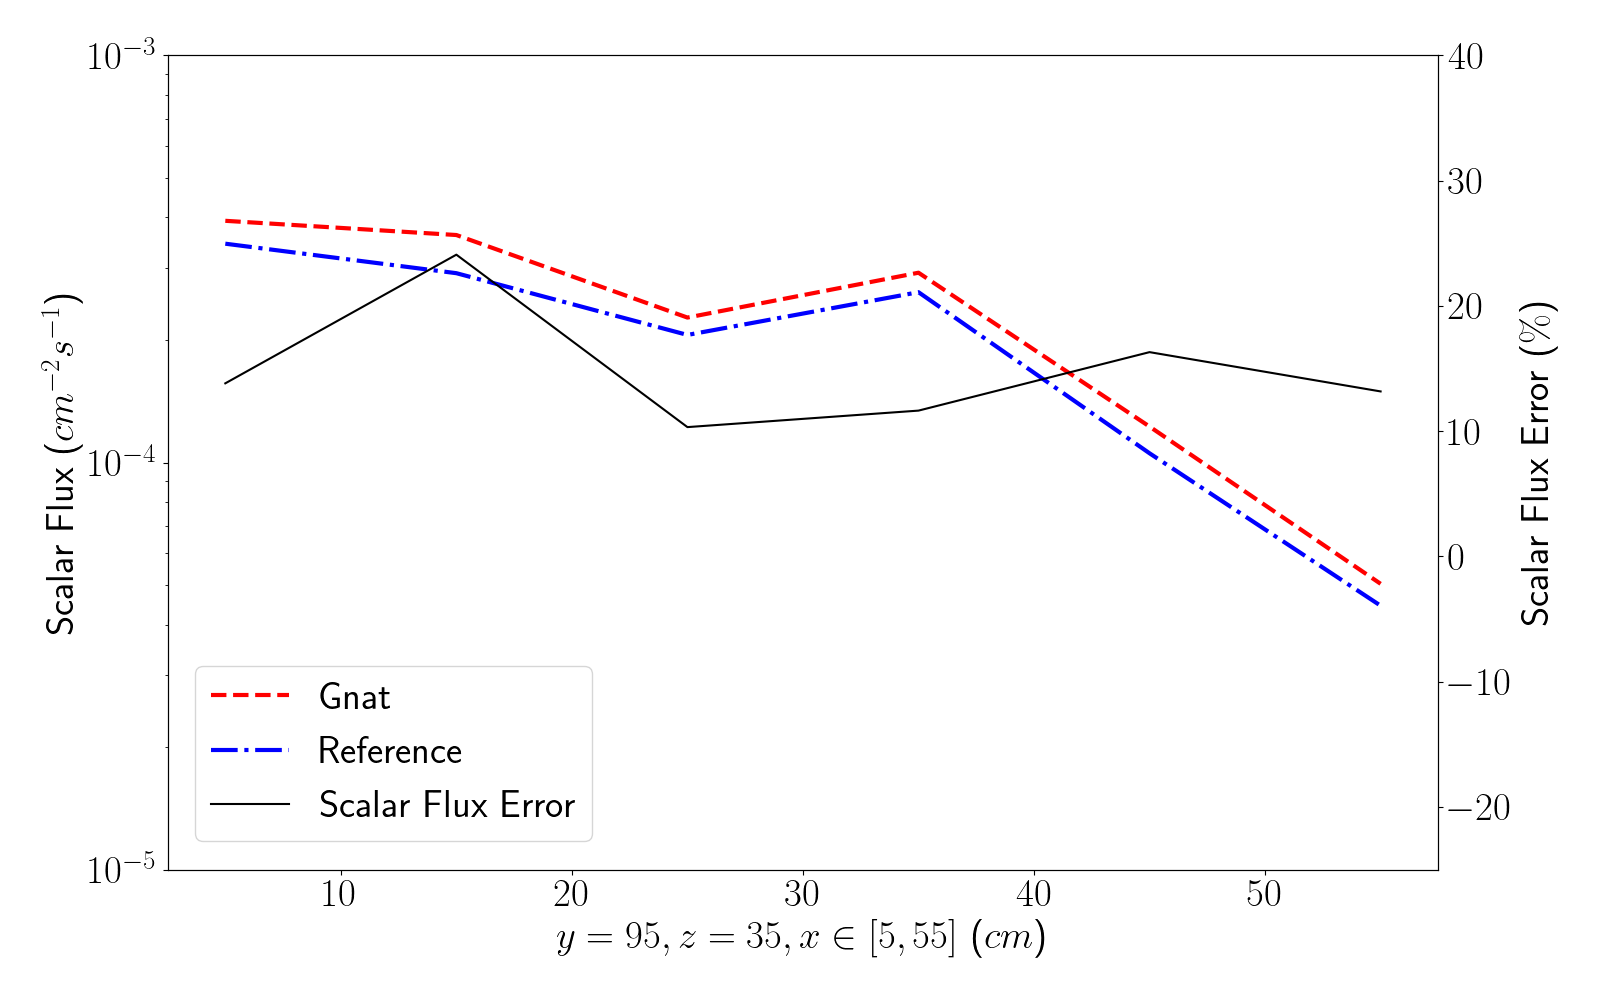
\includegraphics[width=0.8\textwidth]{images/verification/rt_kobayashi/kobayashi_3c_rt.png}
        \caption{With ray effect mitigation. Reference taken from Kobayashi and Sugimura \cite{kobayashi_benchmarks}.}
        \label{fig:verification:rt:kobayashi_3c:rt}
    \end{subfigure}
    \caption{Ray effect mitigation applied to the third Kobayashi benchmark, case c.}
    \label{fig:verification:rt:kobayashi_3c}
\end{figure}
\clearpage

\section{The Self-Adjoint Scalar Flux Approach}
\label{verification:radiation_transport_sasf}

The novel \acrshort{sasf} approach developed in this work was verified with a modified form of the third Kobayashi benchmark. The scattering cross section is set to zero to evaluate a pure absorber problem. As the \acrshort{sasf} technique does not support volumetric or surface sources the source in region one of the Kobayashi benchmark is set to zero. In its place a point source is placed at the origin with an emission rate of $1$ s\textsuperscript{-1}. As there is no existing reference solution to this problem, the method of ray tracing is used to compute scalar fluxes at the element centroids of a 1,474,560 element mesh generated with uniform cube elements. The numerical solution computed with the \acrshort{sasf} method is then sampled at the element centroids of the mesh used for ray tracing for the purposes of computing the relative error. The numerical solution to this problem is computed on a mesh with 1,641,551 nonuniform tetrahedral elements with an average $h$ of 1.131 cm. The region which previously contained the volumetric source is selected as the near-source region for the purposes of removing the singularity in the \acrshort{sasf} equation. The finite element basis functions used were linear Lagrange functions. This case used the \acrshort{pjfnk} solver with preconditioning provided by the hypre package BoomerAMG and 30 \acrshort{gmres} vectors. The initial residual vector magnitude was found to be $1.416106\times 10^{-4}$, and so a relative convergence criteria of $10^{-8}$ is required to ensure that false convergence is not reached at a final residual vector magnitude of $10^{-8}$. 

The results of this problem can be found in Figure~\ref{fig:verification:sasf:z5} for the case where $z = 5$ cm, and the results for the $z = 35$ case can be found in Figure~\ref{fig:verification:sasf:z35}. The largest sources of error occur in three locations: the edges of material discontinuities, the edges of shadows, and the edges of large streaming paths. These are mostly likely caused by large discontinuities in the gradient of the solution perpendicular to the direction of radiation. These errors are severe in this 3D case due to the complexity of the geometry and the addition of surfaces which yield jump discontinuities. Adaptive mesh refinement may be effective for mitigating these errors in problems with highly heterogeneous geometry. Aside from these sources of error the remainder of the error is largely unstructured over the domain. This is likely caused by small changes in the element density across the non-uniform mesh, yielding small fluctuations in error. In general, the numerical solution is free of ray effect and matches the reference solution quite well over the majority of the computational domain.

% 0.325
\begin{figure}[H]
    \centering
    \begin{subfigure}[b]{0.47\textwidth}
        \centering
        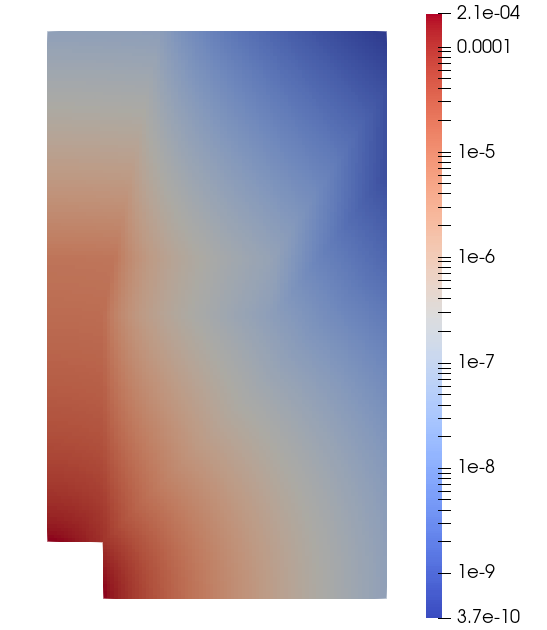
\includegraphics[width=\textwidth]{images/verification/sasf_kobayashi/rt_z5.png}
        \caption{Reference scalar flux (cm\textsuperscript{-2} s\textsuperscript{-1}).}
        \label{fig:verification:sasf:ref_z5}
    \end{subfigure}
    \hfill
    \begin{subfigure}[b]{0.47\textwidth}
        \centering
        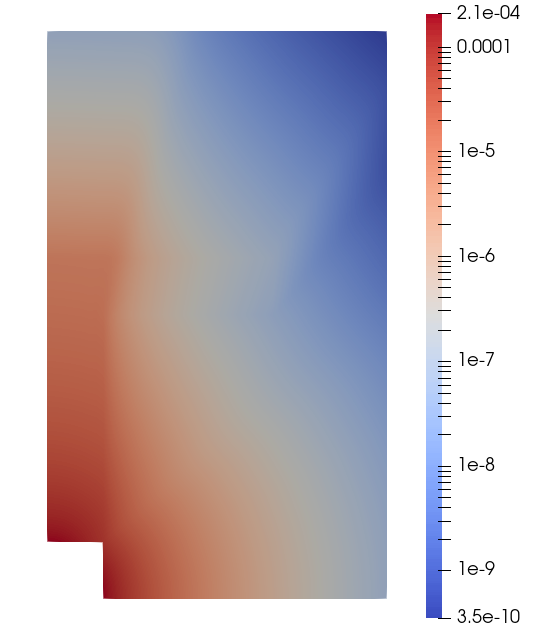
\includegraphics[width=\textwidth]{images/verification/sasf_kobayashi/sasf_z5.png}
        \caption{\acrshort{sasf} scalar flux (cm\textsuperscript{-2} s\textsuperscript{-1}).}
        \label{fig:verification:sasf:sasf_z5}
    \end{subfigure}
    \begin{subfigure}[b]{0.47\textwidth}
        \centering
        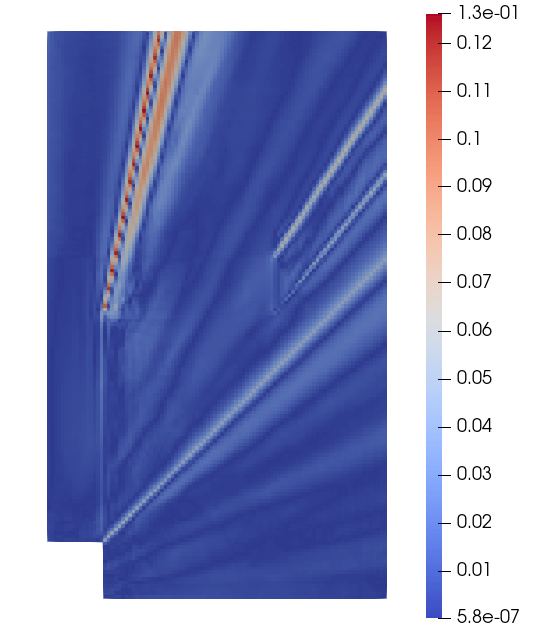
\includegraphics[width=\textwidth]{images/verification/sasf_kobayashi/error_z5}
        \caption{Fractional absolute relative error.}
        \label{fig:verification:sasf:error_z5}
    \end{subfigure}
    \caption{Comparison of scalar fluxes at $z = 5$.}
    \label{fig:verification:sasf:z5}
\end{figure}
\begin{figure}[H]
    \centering
    \begin{subfigure}[b]{0.47\textwidth}
        \centering
        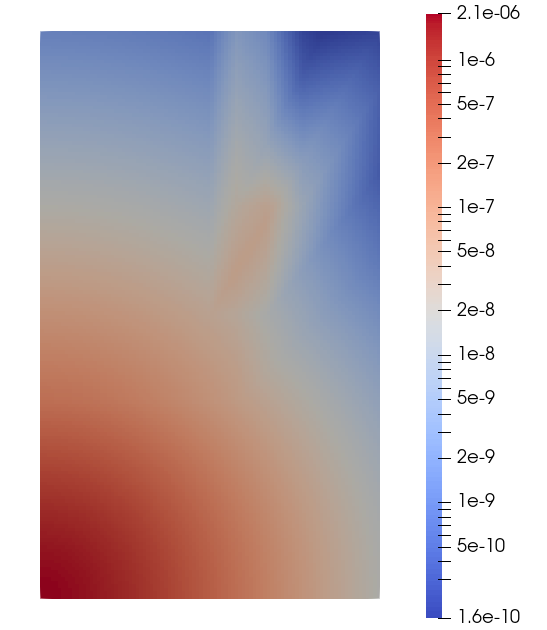
\includegraphics[width=\textwidth]{images/verification/sasf_kobayashi/rt_z35.png}
        \caption{Reference scalar flux (cm\textsuperscript{-2} s\textsuperscript{-1}).}
        \label{fig:verification:sasf:ref_z35}
    \end{subfigure}
    \hfill
    \begin{subfigure}[b]{0.47\textwidth}
        \centering
        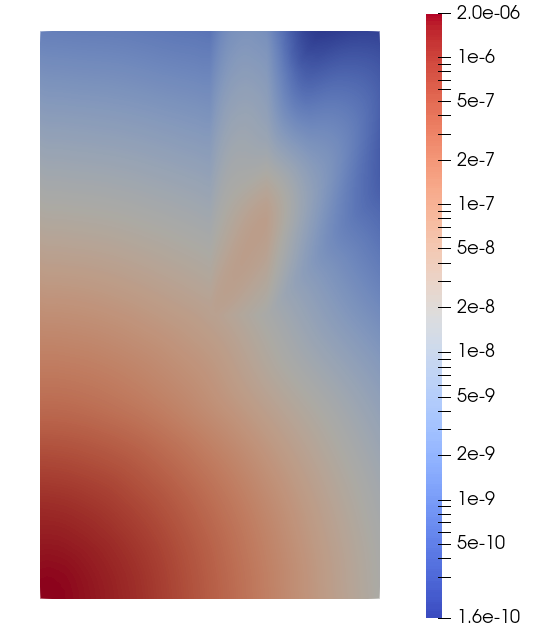
\includegraphics[width=\textwidth]{images/verification/sasf_kobayashi/sasf_z35.png}
        \caption{\acrshort{sasf} scalar flux (cm\textsuperscript{-2} s\textsuperscript{-1}).}
        \label{fig:verification:sasf:sasf_z35}
    \end{subfigure}
    \begin{subfigure}[b]{0.47\textwidth}
        \centering
        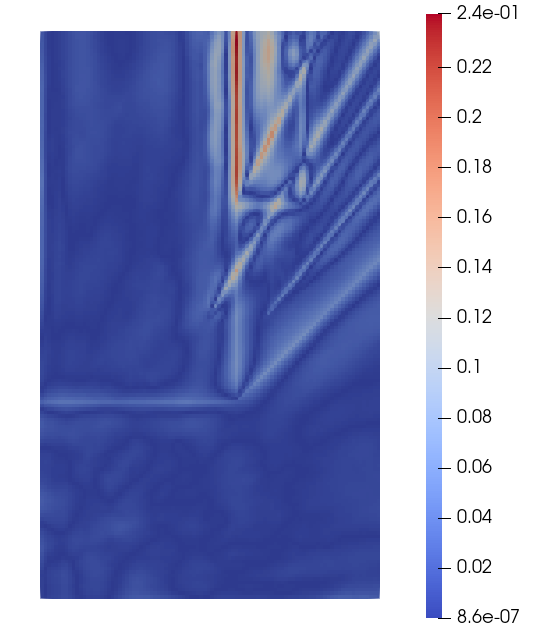
\includegraphics[width=\textwidth]{images/verification/sasf_kobayashi/error_z35}
        \caption{Fractional absolute relative error.}
        \label{fig:verification:sasf:error_z35}
    \end{subfigure}
    \caption{Comparison of scalar fluxes at $z = 35$.}
    \label{fig:verification:sasf:z35}
\end{figure}

\section{The Method of Manufactured Solutions for Mobile Depletion}
\label{verification:mms_mobile_depletion}

The \acrfull{mms} is a verification strategy for partial differential equations similar to comparisons with analytical solutions; it sees an abundance of use for problems which do not have simple analytical solutions in multiple dimensions. The \acrshort{mms} assumes a solution to the governing system of partial differential equations and then computes a forcing function which generates that assumed solution. Consider a radionuclide in a 2D domain under the influence of advection, diffusion, and radioactive decay:
\begin{align}\label{eq:simple_depletion}
    \frac{\partial}{\partial t}N(x,y,t) + \lambda_{i}N(x,y,t) + v_{x}\frac{\partial}{\partial x}N(x,y,t) + v_{y}\frac{\partial}{\partial y}N(x,y,t) = D\Bigg(\frac{\partial^{2}}{\partial x^2}N(x,y,t) + \frac{\partial^{2}}{\partial y^2}N(x,y,t)\Bigg)
\end{align}
where the velocity field $\vec{v}$ and diffusion coefficient $D$ have been assumed to be constant. The \acrshort{mms} can be applied by bringing the diffusion term to the right and setting the resulting expression equal to a forcing function:
\begin{equation}\label{eq:simple_depletion_force}
    \frac{\partial}{\partial t}N(x,y,t) + \lambda_{i}N(x,y,t) + v_{x}\frac{\partial}{\partial x}N(x,y,t) + v_{y}\frac{\partial}{\partial y}N(x,y,t) -D\Bigg(\frac{\partial^{2}}{\partial x^2}N(x,y,t) + \frac{\partial^{2}}{\partial y^2}N(x,y,t)\Bigg) \\= f(x,y,t)\text{,}
\end{equation}
where $f(x,y,t)$ is the forcing function. To verify the implementation of the spatial discretization scheme steady state is assumed and the time derivative is set to zero. The solution is then assumed to take the following form:
\begin{equation}\label{eq:mms_spatial_assumed}
    N(x,y) = e^{xy}\text{.}
\end{equation}
Substituting Eq.~\ref{eq:mms_spatial_assumed} into Eq.~\ref{eq:simple_depletion_force} and simplifying yields the following forcing function:
\begin{equation}
    f(x,y) = xv_{y}e^{xy} + yv_{x}e^{xy} - Dy^2e^{xy} - Dx^2e^{xy} + \lambda e^{xy}\text{.}
\end{equation}
The use of the exponential function over simpler functions such as polynomials is to introduce numerical error into the solution; polynomial basis functions cannot exactly represent the behavior of transcendental functions. This allows for the measure of spatial convergence by using the difference between the numerical solution and the assumed solution.

To measure temporal convergence using the \acrshort{mms} the solution is assumed to be a linear function in space such that it can be exactly represented by linear Lagrange basis functions:
\begin{equation}\label{eq:mms_temp_assumed}
    N(x,y,t) = xyt^3\text{.}
\end{equation}
Substituting Eq.~\ref{eq:mms_temp_assumed} into Eq.~\ref{eq:simple_depletion_force} and solving for the forcing function results in the following:
\begin{equation}
    f(x,y,t) = \lambda xyt^3 + 3xyt^2 + v_{y}xt^3 + v_{x}yt^3\text{.}
\end{equation}

The \acrshort{mms} was applied to both the \acrshort{supg} finite element and \acrshort{fvm} mobile depletion solvers. In the case of the \acrshort{supg} method, linear and quadratic Lagrange basis functions were used. In the case of the \acrshort{fvm}, the first order upwinding and second order van Leer closures implemented in \acrshort{moose} were used. The domain consisted of a 1 cm x 1 cm square meshed with 8 elements on each axis. This mesh was then refined three times to measure the $L_{2}$ error of solutions at different mesh resolutions. As these problems are relatively small and the Jacobians used by the mobile depletion solver are exact due to the use of \acrshort{ad}, the Newton solver was used with an absolute tolerance of $10^{-12}$ and a relative tolerance of $10^{-8}$. The resulting $L_{2}$ error for the spatial cases is plotted in Figures~\ref{fig:verification:dep:spatial} against the average element size ($h$) for when $D = 1$, $v_{x} = 1$, $v_{y} = 1$, and $\lambda = 1$. The temporal case used linear Lagrange basis functions (\acrshort{supg}) and first order upwinding (\acrshort{fvm}) on the most refined mesh from the spatial case. A $\Delta t$ of 1 s was used, which was then uniformly refined three times to measure temporal convergence over different time steps. The results for when $D = 1$, $v_{x} = 1$, $v_{y} = 1$, and $\lambda = 1$ can be found in Figure~\ref{fig:verification:dep:temp}. In all cases Dirichlet boundary conditions are applied on all sides with the forcing function as the value.

\begin{figure}[H]
    \centering
    \begin{subfigure}[b]{\textwidth}
        \centering
        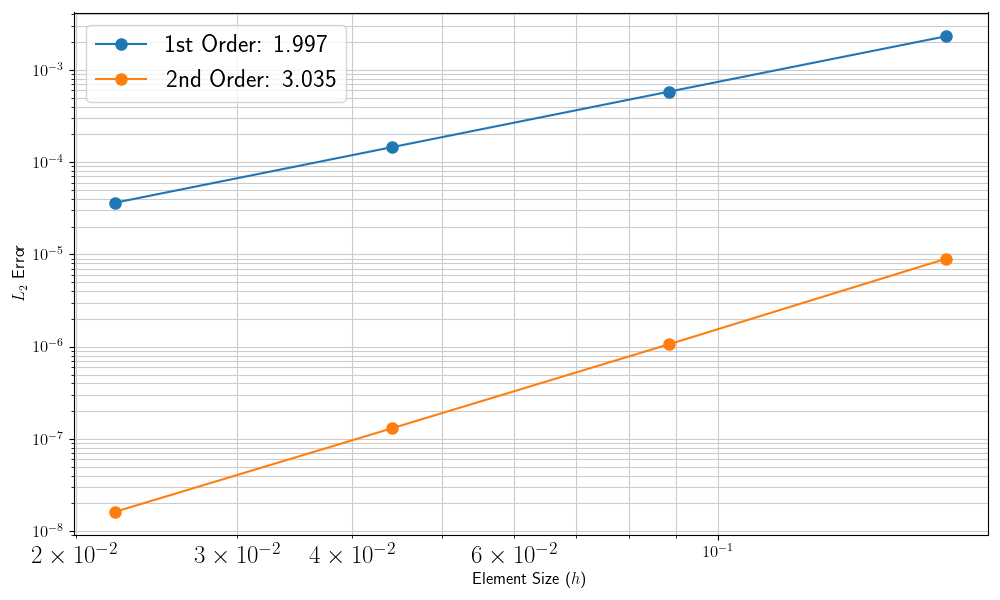
\includegraphics[width=0.8\textwidth]{images/verification/depletion/nuclide_mms_spatial_fe.png}
        \caption{\acrshort{supg} solver.}
        \label{fig:verification:dep:spatial:fe}
    \end{subfigure}
    \hfill
    \begin{subfigure}[b]{\textwidth}
        \centering
        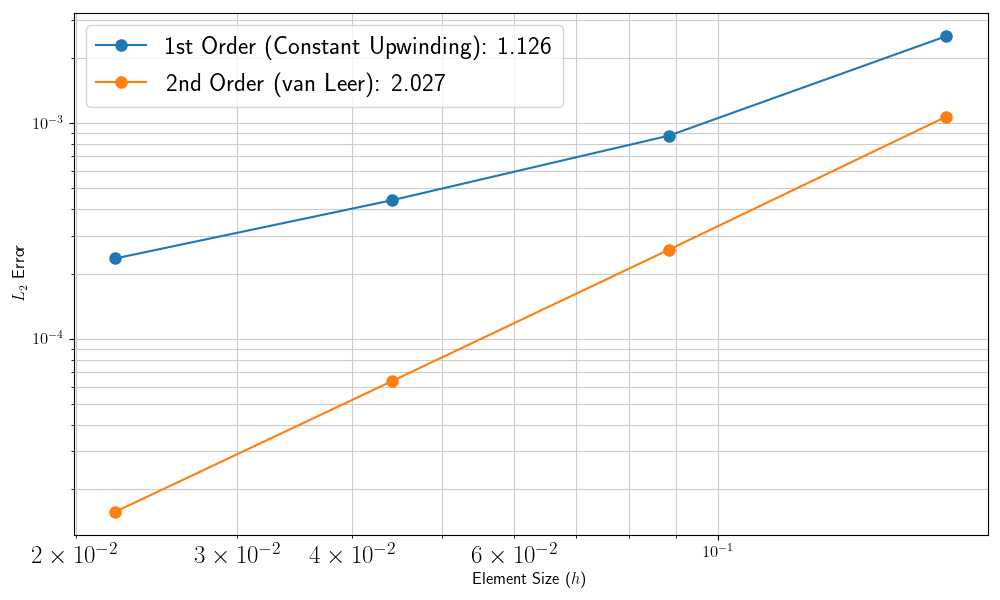
\includegraphics[width=0.8\textwidth]{images/verification/depletion/nuclide_mms_spatial_fv.png}
        \caption{\acrshort{fvm} solver.}
        \label{fig:verification:dep:spatial:fv}
    \end{subfigure}
    \caption{Spatial verification of the mobile depletion solver using the \acrshort{mms}.}
    \label{fig:verification:dep:spatial}
\end{figure}

\begin{figure}[H]
    \centering
    \begin{subfigure}[b]{\textwidth}
        \centering
        \includegraphics[width=0.8\textwidth]{images/verification/depletion/nuclide_mms_temp_fe.png}
        \caption{\acrshort{supg} solver.}
        \label{fig:verification:dep:temp:fe}
    \end{subfigure}
    \hfill
    \begin{subfigure}[b]{\textwidth}
        \centering
        \includegraphics[width=0.8\textwidth]{images/verification/depletion/nuclide_mms_temp_fv.png}
        \caption{\acrshort{fvm} solver.}
        \label{fig:verification:dep:temp:fv}
    \end{subfigure}
    \caption{Temporal verification of the mobile depletion solver using the \acrshort{mms}.}
    \label{fig:verification:dep:temp}
\end{figure}

In the case of the \acrshort{supg} solver, the convergence tests result in the expected convergence behavior for first order and second order elements. In the case of spatial convergence the $L_{2}$ error should decrease as a function of $h^{M_{s}+1}$, where $M_{s}$ is the order of the element. The calculated values of $M_{s}+1$ using linear regression can be found in the legend of Figure~\ref{fig:verification:dep:spatial:fe}, where it approaches the true value for both first and second order elements; second and third order convergence in the $L_{2}$ norm respectively \cite{finite_element_method}. When it comes to temporal convergence the $L2$ error should decrease as a function of $\Delta t^{M_{t}}$, where $M_{t}$ is the order of the time integration scheme. The calculated value of $M_{t}$ using a linear regression can be found in the legend of Figure~\ref{fig:verification:dep:temp:fe}, where it approaches the true value for both first order implicit Euler and second order backwards difference schemes. The convergence test also resulted in the expected behavior for the \acrshort{fvm} solver. In the spatial case, first order upwinding should result in first order convergence, and second order van Leer closures should result in second order convergence \cite{finite_volume_methods}. This is observed in the legend of Figure~\ref{fig:verification:dep:spatial:fv}. The temporal convergence of the \acrshort{fvm} solver should match that of the \acrshort{supg} solver as the same time integrators are used for both; this can be seen in Figure~\ref{fig:verification:dep:temp}. 

\section{Summary}
\label{verification:summary}
The implemented radiation transport and mobile depletion solvers have been compared to a suite of problems. These included analytical solutions to the underlying governing equations, standard benchmark problems, novel benchmark problems, and the \acrshort{mms}. The \acrshort{sn} transport solver was found to converge to a simple 1D analytical solution to the transport equation as the spatial and angular domain was progressively refined. The \acrshort{sn} solver was also found to agree well with all three of the Kobayashi benchmarks and the Ontario Tech subcritical assembly benchmark. There were limits on the accuracy that the solver was capable of obtaining due to the coarse meshes used due to computational constraints; all simulations were ran on a single 64 core compute cluster with 256 GB of RAM. The ray traced uncollided flux method was found to converge to the expected solutions to the transport equation in the case of a simple 3D problem, and it was also capable of mitigating ray effects in the third Kobayashi benchmark when a low order angular quadrature set was used for the collided flux. The \acrshort{sasf} approach was found to be accurate when solving a modified version of the third Kobayashi problem, although there are limitations when it comes to the current implementation of the technique which prevented it from being used for the full benchmark problem. Finally, the mobile depletion solvers were verified using the \acrshort{mms} where the expected order of spatial and temporal convergence was found for both the \acrshort{supg} approach and the \acrshort{fvm} solvers. The success of these verification problems indicate that the implementation of the governing equations in \acrshort{gnat} is correct.